

\chapter{Nbody application}
\label{Chap:nbody}

After the previous analytical study, we present here the characteristics of numerically obtained Hubble-Lema\^itre fragmented models. We describe the integrator NBODY6 and data analysis framework StarFiddle, as well as a clump-finding algorithm that we use to analyse the population of clumps obtained from the expansion. We investigate the influences of N, \tHub and stellar mass functions on the clumps mass function. We then look at the stellar content and distribution inside clumps, comparing them to clumps obtained from hydrodynamical simulations.


\minitoc



\begin{figure}
\begin{center}
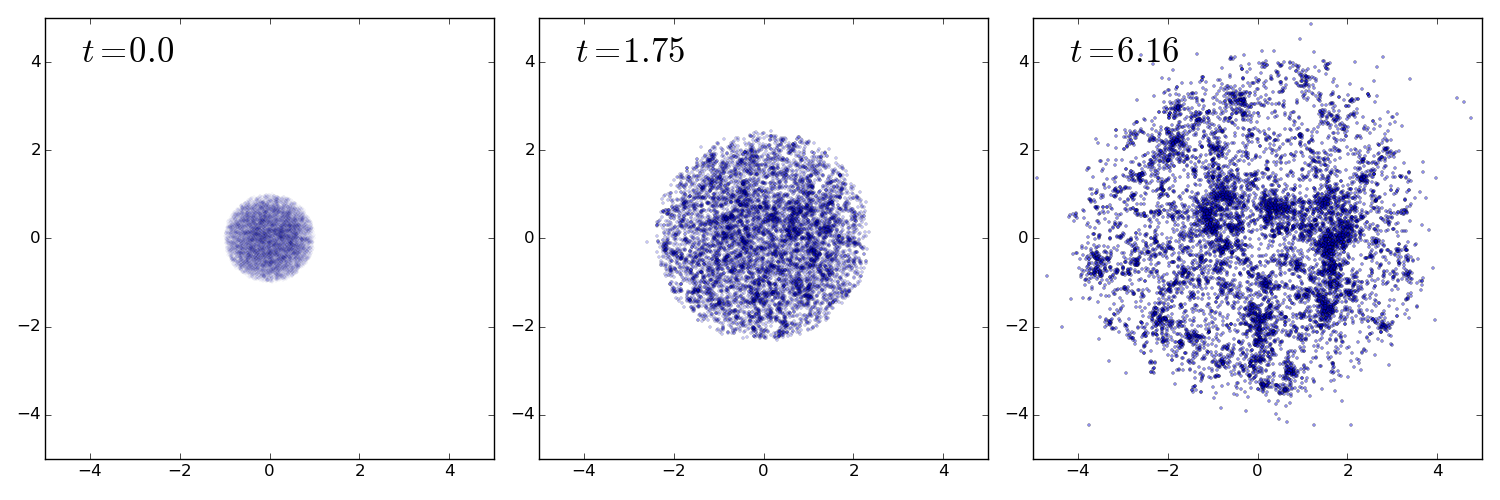
\includegraphics[width=\textwidth]{Figures/2_fragmentation}
\caption[Fragmentation of a \HubLem model]{Progressive fragmentation through the Hubble expansion. The left panel shows the initial uniform sphere; the middle panel, an intermediate step, slightly fragmented with a slowed down expansion; the right panel is the final stage, when the expansion has stopped and the fragmentation is fully developed. N=10000 particles were used in this N-body model, with $\Hub_0 = 1.0$. Time and coordinates are in H\'enon units.}
\label{Fig:2_fragmentation}
\end{center}
\end{figure}




\section{Numerical tools}

\subsection{H\'enon units}


Many N-body integrators use a set of units specifically invented for the N-body gravitational problem, the N-body units, or H\'enon units (as prescribed by Douglas Heggie during the MODEST 2014 meeting). They were introduced by \cite{Henon1971} and are based on three relations:

\begin{align}
G &= 1\\
M_t &= 1\\
E &= -\frac{1}{4}
\end{align}

With $G$ the gravitational constant, $M_t$ the total mass of the system and $E$ total energy of the system. For a virialized system, that is a relaxed system in which the virial ratio 
\begin{equation}
Q = - \frac{E_k}{E_p} = 0.5,
\end{equation}
it comes that $E_k=0.25$ and $E_p = -0.5$ and, considering the definition of the virial radius 
\begin{equation}
R_v = - \frac{G M_t^2}{2 E_p} = 1.
\end{equation} 

This unit system was designed for virialized systems, but can be used for out of equilibrium systems, as long as they are bound ($Q <1$), with energy expressions functions of $Q$
\begin{align}
E_p  &= - \frac{1}{4(1-Q)}\\
E_k &= \frac{Q}{4(1-Q)}
\end{align}
which still fulfills the $E = -\frac{1}{4}$ condition. In practice, the H\'enon mass, radius and velocities are obtained through

\begin{align}
m_h &= \frac{m}{M_t}\\
r_h &= 4 (1-Q) |E_p| \cdot r\\
v_h &= \sqrt{ \frac{Q}{4(1-Q) E_k} } \cdot v
\end{align}

with $E_p$ and $E_k$ being computed with H\'enon masses and $G=1$ but before rescaling length and velocities. Such a system can be used as an input for NBODY6 without the need for the software to rescale anything, as NBODY6 internally works with H\'enon units.


\subsection{NBODY6}


NBODY6 is a N-body integrator. It computes the trajectories in a system of interacting point masses. It is the second youngest iteration of the NBODY family, a suite of N-body integrators created by Sverre Aarseth. It can compute the gravitational interaction between up to 128,000 stars in a collisional fashion, meaning there is no softening of the potential, at any scale. This allows for very close binaries to form and remain in the system. The code preserves the total energy and angular momentum to better than one part in $10^4$ for integration over $\sim 100 $ time units.

To achieve its impressive performances, NBODY6 relies on several optimization technique which have been first developed in the 1960s and 1970s, and improved ever since. NBODY1, first of its name, was developed in the early 1960s and based on the idea of force polynomial fitting: to ensure convergence, trajectories were computed by fitting polynomials to forces and obtaining high-order derivatives. Over time, the force fitting was enhanced, and additional techniques were added over the versions: NBODY3, NBODY2, NBODY4, NBODY5 (in that order, see \citealt{Aarseth1999} for a summary of the NBODYs development).

NBODY6 was a work-station version of NBODY5 and was first developed throughout the 1990s. It has been enhanced and optimized ever since. It inherited the major features from its NBODY ancestors that made them so successful. They are briefly described here in chronological order of their implementation:

\begin{itemize}
\item[\textbf{block time-steps;}] very early on, particles were attributed individual time-steps, functions of their acceleration. An innovation was to commensurate these time-steps: they could only be reduced by factors of 2, so all particles could easily resynchronise at some point in the simulation;

\item[\textbf{KS-regularization}] was introduced to circumvent the large acceleration in close pairs that slowed down integration, it relies on a change of variables for the pair that makes its integration faster, while still factoring perturbing influence from other particles; 

\item[\textbf{Ahmad-Cohen Neighbour scheme;}] considering that close neighbours and distant particles have distinct dynamical effects, their influences were split into regular and irregular integrations, with some level of synchronization;

\item[\textbf{Hermite integration scheme}] was introduced as the latest integration scheme in the NBODY codes, it allows to obtain high-order estimates of future positions and velocities with limited computational cost.

\end{itemize}

Appendix~\ref{App:nbody6} contains additional details on these optimization techniques and a complete description can be found in Sverre Aarseth's book \citep{Aarseth2003}.

While a new generation, NBODY7, was developed to include post-newtonian effects and correctly integrate black hole binary dynamics \citep{Aarseth2003b}, the NBODY6 family has been extended into several branches. \cite{Spurzem1999} developped Nbody6++, a parallel version powered by MPI, while \cite{Nitadori2012} developed NBODY6GPU, a GPU-accelerated version. Recently, both versions were merged into a MPI-GPU hybrid NBODY6++-GPU \citep{Wang2015}. \cite{Renaud2011} and \cite{Renaud2015} introduced Nbody6tt, which allows the inclusion of complex tidal fields from large-scale galactic simulations.

In this work, we adopted the widely used "vanilla" version NBODY6, and its GPU accelerated version when the number of particles exceeded 3000 (from several performance tests on our models).



\subsection{StarFiddle, an N-body API}



\begin{figure}
\center
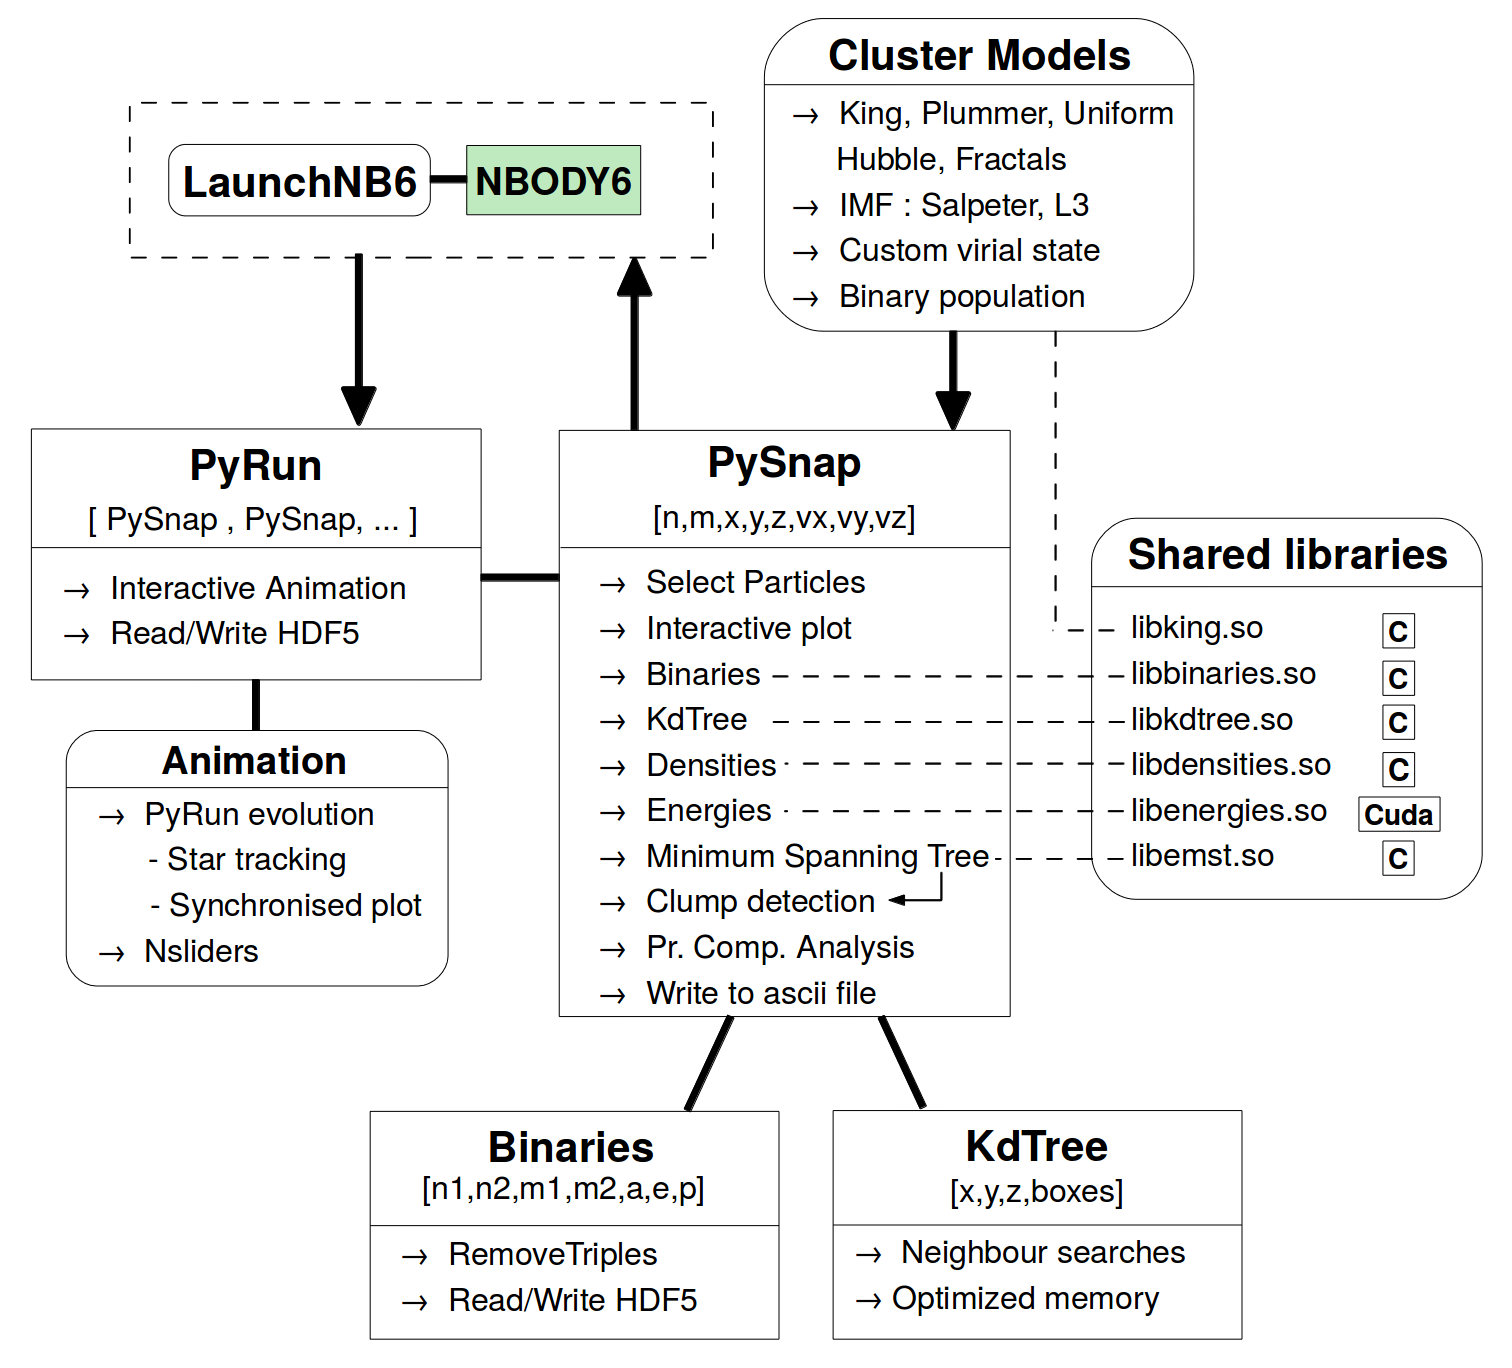
\includegraphics[width=\linewidth]{Figures/0_StarFiddle}
\caption[Visualization of the StarFiddle API]{Visualization of the StarFiddle API. Squared boxes are data storing classes while rounded boxes are modules.}
\label{Fig:0_StarFiddle}
\end{figure}


Over the course of this work, I developed several python interfaces and modules to handle snapshots of N-body simulations. Several C and Cuda libraries were implemented in these modules. Finally, all these were unified as a N-body python API called StarFiddle.

StarFiddle is centered around the PySnap class, which stores information about a N-body simulation snapshot: identities of particles (n), masses, position and velocities. This class has a wealth of methods to perform various analysis. The main methods are:

\begin{itemize}
\item Interactive Plot - 3d interactive and customizable 3D representation;
\item SelectParticles - allows boolean selection to produce a PySnap of a subsample;
\item Binaries - detects binary stars using the algorithm described in chapter \ref{Chap:BinAlgo};
\item kdTree - builds a kdTree of the spatial distribution to perform neighbour searches;
\item Densities - computes local densities for each particles through the kdTree;
\item Energies - computes individual potential and kinetic energies for all particles;
\item Minimum Spanning Tree - builds the MST of the system, for structure analysis;
\item Clump detection - extracts overdensities through the algorithm described in next section;
\item Principal Component Analysis - performs a PCA on the system for structure analysis;
\item Write to file - writes the data to an ASCII file.
\end{itemize}

Computationally intensive algorithms were written in C or Cuda, then compiled into shared libraries. These can be called from C or Python through the ctypes module. The binary, energy and density algorithm were fully written for StarFiddle. The kdTree algorithm was adapted from C++ from \cite{numericalrecipes} to C, and its memory use was optimized; the algorithm was successfully ran on cosmological simulations for 280 million points. The minimum spanning tree was provided by the \href{http://mlpack.org/}{MLPACK library}. Binaries and kdTree are classes of their own which allows easy data storage and management.

The Cluster Models module lets the user create PySnap instances of various models of star clusters: King, Plummer, Uniform, Fractal or Hubble. The King model uses a C implementation of a fortran algorithm by Gerry Quinlan and Christian Boily. The models can be set to arbitrary virial parameters $Q$ and injected with primordial binary populations. The stars can have identical masses or follow a Salpeter or L3 Initial Mass Function (\textbf{IMF}) with user-provided parameters.

LaunchNB6 is a Python interface for NBODY6. I slightly modified NBODY6 so it prints ASCII snapshot files in place of the regular binary format output. LaunchNB6 creates the specified working directory and launch the integration from initial conditions, either a specific PySnap, or one created from the Cluster Models. It then reads the snapshot files to create a PyRun instance. A PyRun can be stored and retrieved from a HDF5 file. This instance is strongly related to the Animation module.

The Animation module allows interactive 3D animation of a PyRun and the creation of synchronized plots to follow related data during the evolution. A specified subset of stars can be marked and follow during the animation. In addition to PyRun, Animation lets the user create interactive plots with an arbitrary number of sliders to easily explore a parameter space.

StarFiddle is available on \href{https://github.com/dorvaljulien/StarFiddle}{GitHub}.












\subsection{Clump finding algorithm}

As seen on Fig~\ref{Fig:2_fragmentation}, once expansion stops, the distribution is roughly spherical and visibly clumpy. By clump we mean here a local overdensity of stars. To characterize the model, it is necessary to find and isolate clumps, using an efficient clump-identification algorithm (or, {\it halo-finding} in cosmology).  Several methods are commonly used, such as the HOP algorithm \citep{Eisenstein1998,Skory2010} which relies on attributing local densities to each particle and separating the clumps through density thresholds. The HOP algorithm is very robust on large cosmological data sets. However, our calculations have comparatively coarse statistics and noisy density fields. This issue, coupled with the  large number of free parameters of the HOP algorithm, makes the method less appealing. 

Instead we follow \cite{Maschberger2010} who adapted the minimum spanning tree (MST~; see e.g. ~\citealt{Allison2009b,Olczak2011}) technique to the detection of clumps. A spanning tree is a set of edges connecting a group of  particles without closed loops~; the MST seeks to minimise the total length of the edges. One may then construct the MST for the whole system, then delete all edges larger than a chosen cutting length, $d_{cut}$. The sub-sets that are still connected  are labelled as clumps. This process is illustrated in Fig \ref{Fig:2_MST}. In practice a minimum sub-set size $N_d$  is also chosen so as to avoid many small-N subgroups: experience led us to choose  $N_d = 12$ for the minimum number of stars per clump. 

\begin{figure}
\begin{center}
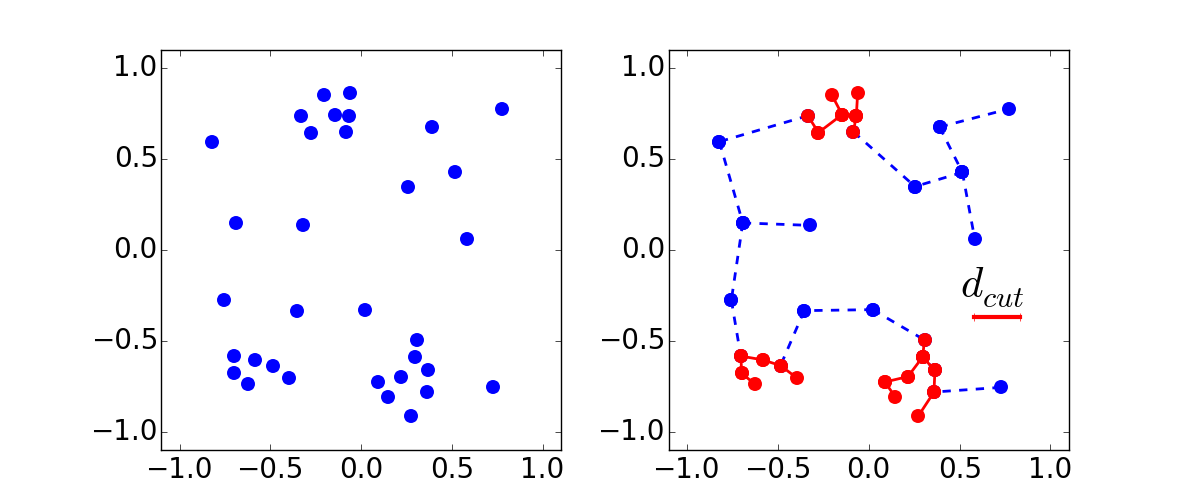
\includegraphics[width=0.8\columnwidth]{Figures/2_MST.png}
\end{center}
\caption[Illustration of a Minimum Spanning Tree and its use to isolate subgroups]{Illustration of a Minimum Spanning Tree and its use to isolate subgroups, using a cutting length $d_{cut} = 0.25$ length units.}
\label{Fig:2_MST}
\end{figure}


With $N_d$ fixed, the length $d_{cut}$ is then the only free parameter left. There is some freedom 
in choosing an appropriate value. \cite{Maschberger2010} fixed the value of  $d_{cut}$ by visual inspection of clumps.  We instead  identified  clumps in a fragmented system for a range of values for $d_{cut}$ and settled for the value  which optimised the number of identifications. This is shown on Fig.~\ref{Fig:2_Ndcut} for the fully-fragmented state of a N=80k \HubLem model. For small values of $d_{cut}$, the number of detected clumps at first  increases rapidly. The rise is due  to the length $d_{cut}$ initially being small compared with the typical volume spawned by $N_d$ or more  nearest-neighbours. Beyond a certain value, a transition to another regime occurs, whereby the algorithm starts to connect previously separated clumps, counting them as one. The number of clumps thereafter begins to decrease. The value $d_{cut} \approx 0.023$ H.u optimises the outcome of the clump-search. This is a generic feature of the MST algorithm and we have adopted the same strategy throughout, adapting the value of $d_{cut}$ to the number $N$ of stars used. 





\begin{figure}
    \centering
    \begin{subfigure}[b]{0.49\textwidth}
    	\centering
    	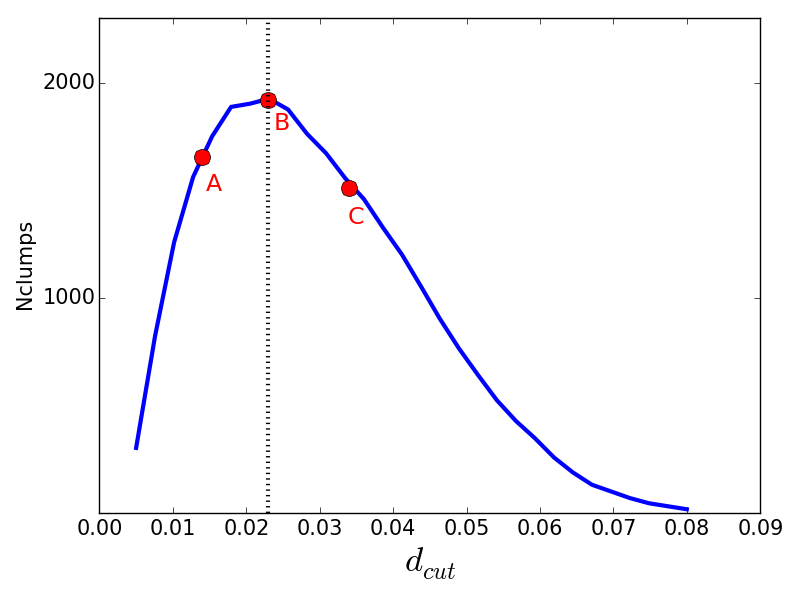
\includegraphics[width=\textwidth]{Figures/2_Ndcut.png}
        \caption{Number of clumps vs $d_{cut}$}
        \label{Fig:2_Ndcut}
    \end{subfigure}
    \begin{subfigure}[b]{0.49\textwidth}
    	\centering
    	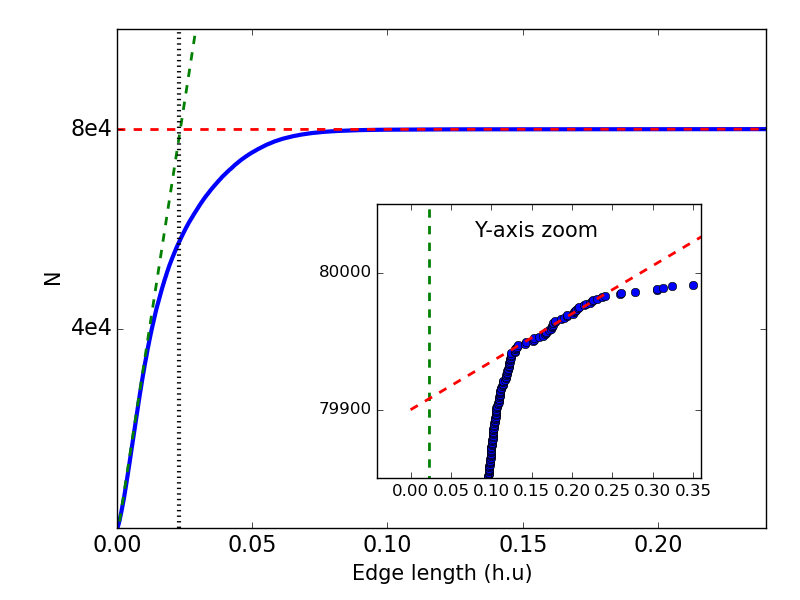
\includegraphics[width=\textwidth]{Figures/2_dcutdistribution.png}
        \caption{Cumulative distribution of MST edges}
        \label{Fig:2_dcutcumulated}
    \end{subfigure}
\caption[Two different methods to identify the critical $d_{cut}$ for clump detection]{Two different methods to identify the critical $d_{cut}$ for clump detection. Both methods give the same value. For this 80k model, the value is 0.023 in H\'enon units. The red linear fit on (b) was made on the linear portion of the distribution, discarding the seven further points departing from the tendency.}
\label{Fig:0_dcutchoice}
\end{figure}


 

 


\begin{figure}
\begin{center}
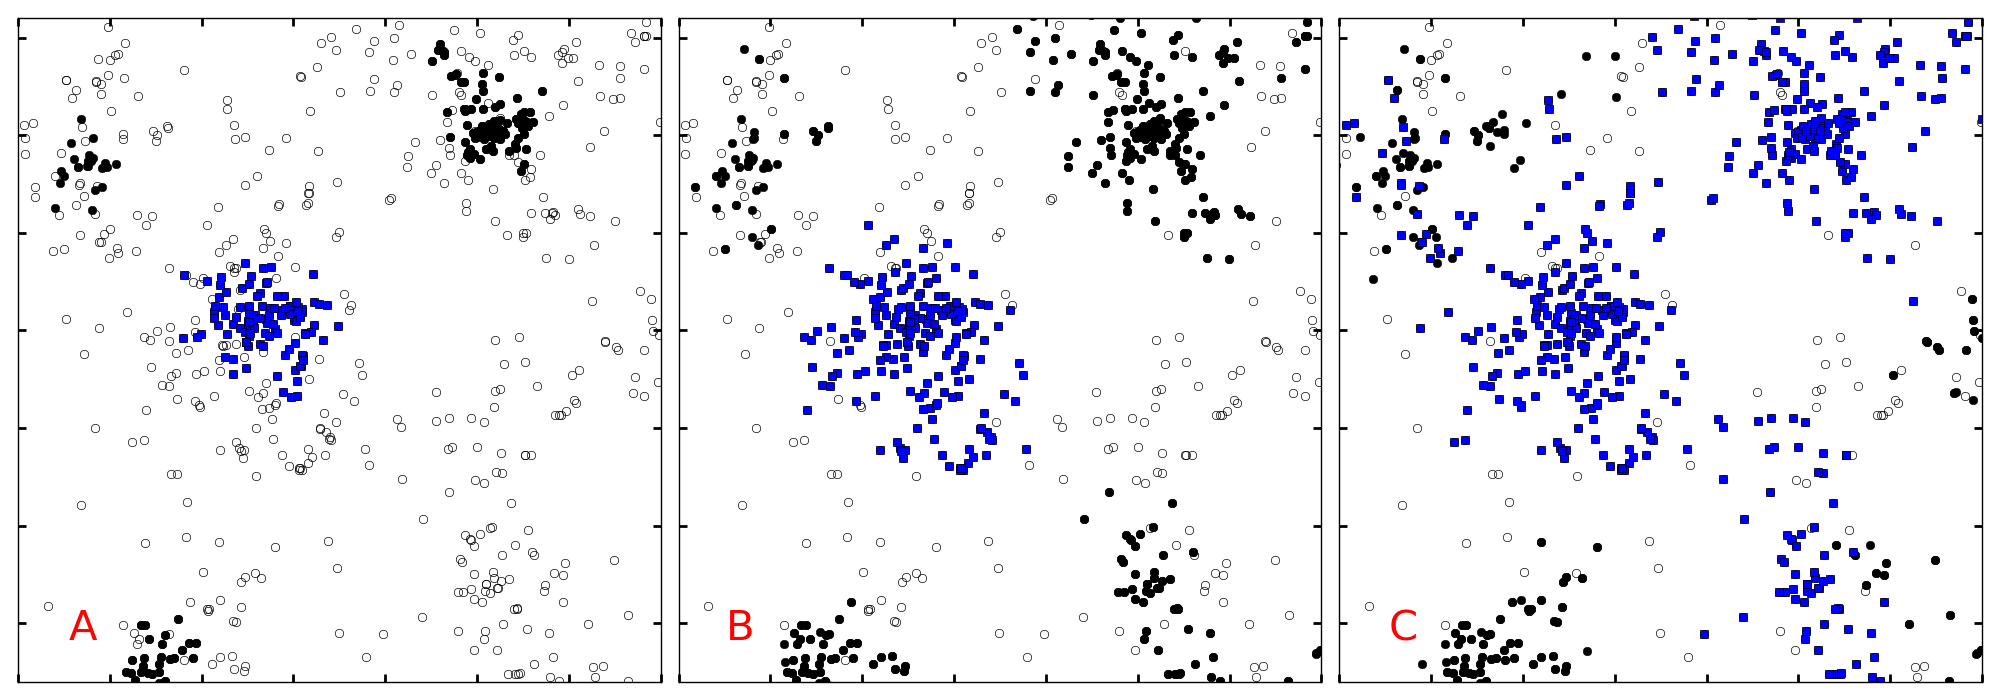
\includegraphics[width=\columnwidth]{Figures/2_clumpsABC.png}
\end{center}
\caption[Example of detected clumps for three cutting lengths in a N=80k model]{Example of detected clumps for three cutting lengths, 0.013 (left panel), 0.023 (middle panel), 0.033 (right panel), which were labeled A,B,C  in Fig.~\ref{Fig:2_Ndcut}. A cube within the N=80k particles fragmented model was extracted and projected.  Empty circles are stars which do not belong to any clump, black circles are clump members, and blue squares are stars that are identified as a single large  clump. Tick marks are spaced by 0.05 length units for a box size of 0.35 units.}
\label{Fig:2_clumpsABC}
\end{figure} 




Another method to find the critical cutting length was used by \cite{Gutermuth2009,Kirk2011}. In these works, the authors build the MST, then trace the cumulative distribution function of all edges in the tree. In a clumpy configuration, there are at least two regimes: the "intra-clump" regime, with the majority of small edges, and the "inter-clump" regime with longer, scarcer edges. The intersection of the linear fits to these regimes provide a good cutting length for clump detection. This procedure was applied to our system and gave the same result than the clump count, as shown on Fig~\ref{Fig:2_dcutcumulated}.

 
   On Fig.~\ref{Fig:2_clumpsABC}, a sub-set of the N=80k model is shown; we have identified stars that belong to clumps with filled symbols. The three panels on that figure are each for a different value of $d_{cut}$, increasing from left to right. For the smallest value $d_{cut}$=0.013 H.u, clumps look somewhat truncated as we are still in the under-sampling regime and only their cores registered as clumps. The second, optimal, value $d_{cut}$=0.023 H.u produces visually well-isolated clumps. Finally, the third and  largest value is so that clumps begin to merge together~: this is shown by the unique clump identified in the bottom panel (filled blue squares).
   
   
   
\begin{figure}
\begin{center}
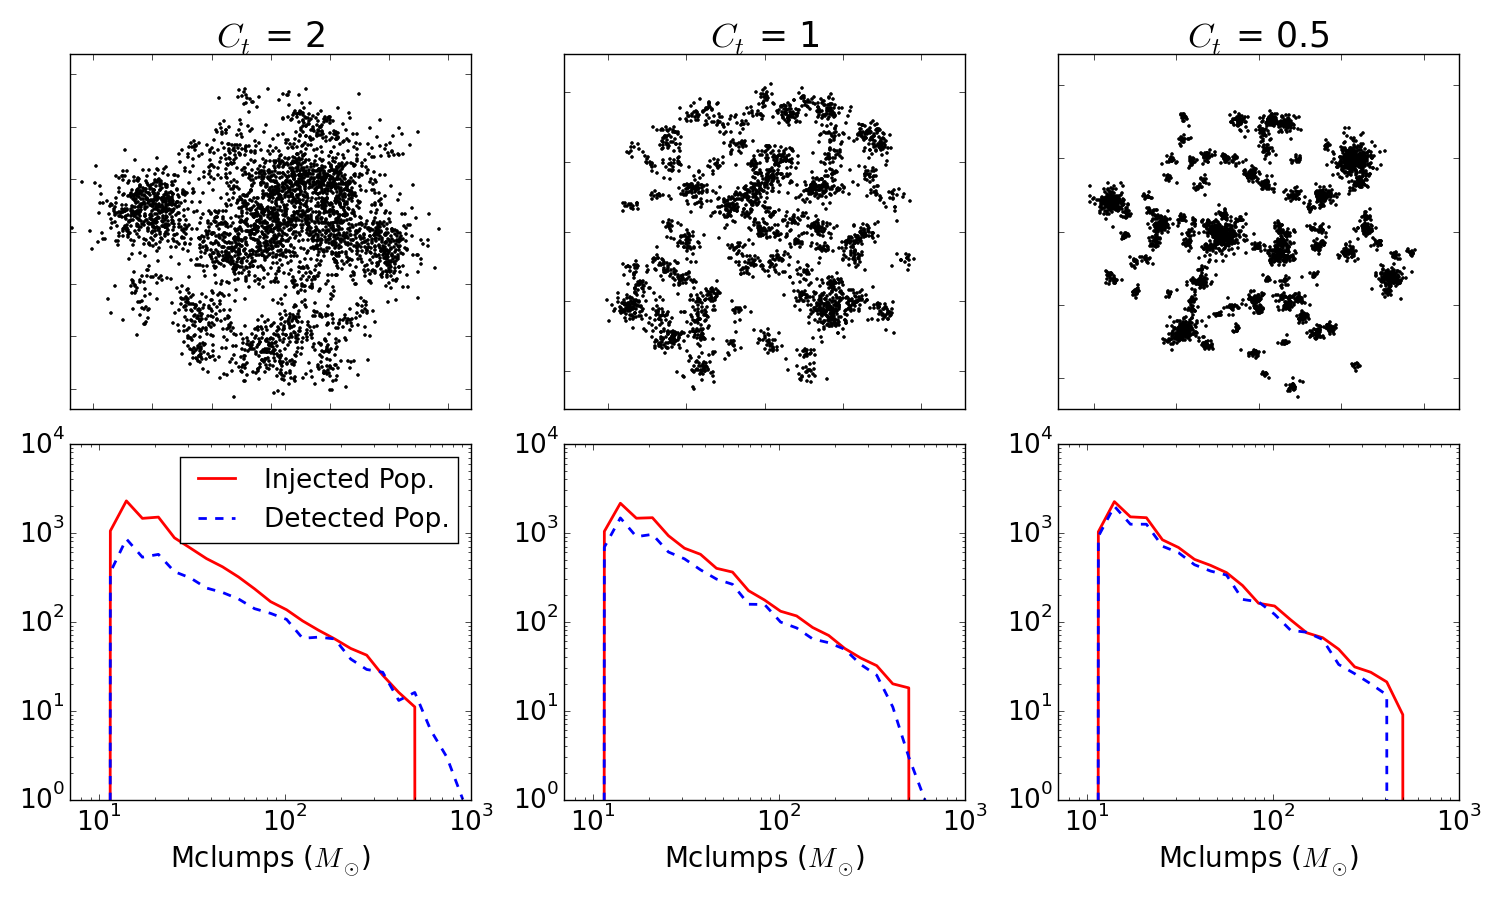
\includegraphics[width=0.9\textwidth]{Figures/2_clumpcheck.png}
\caption[Retrieval of a known clump mass function to test the algorithm]{Top panels: spatial distribution of stars in systems with various compactness factors $C_t$. Bottom panels: clump mass function for the population injected in the system in solid red and the population returned by the clump finding algorithm in dashed blue.}
\label{Fig:2_clumpcheck}
\end{center}
\end{figure} 



   
   To check whether this algorithm is able to efficiently retrieve a clump mass function, I performed an additional test. Several artificially substructured models were created through the Plummer scatter method (see section \ref{Sec:0_substructure}). A multitude of Plummer spheres were generated following a L3 IMF for both the clump  and stellar masses. All clumps radii were scaled so they all had similar number densities. The clumps were placed in space following a uniform distribution. We wish to explore the algorithm behaviour with varying ``clump crowding". In a spherical uniform distribution of radius 1, the mean nearest-neighbour distance is expressed as
 
\begin{equation}
\langle d_{nb}\rangle \simeq 0.8 N^{-\frac{1}{3}} .
\end{equation}
   
See \cite{Chandrasekhar1943} for details. We compute the average 90\% Lagrangian radius of our Plummer clumps, $\langle R_{90}\rangle$, then introduce the compactness factor

\begin{equation}
C_t = \frac{ 2 \langle R_{90}\rangle}{\langle d_{nb}\rangle }.
\end{equation}

For $C_t <1$, the clumps are smaller than the interclump distance, while for $C_t > 1$, clumps are in contact and mixed together for high enough values. Once the positions of the uniform distribution are generated, it is possible to scale them to generate a system with a custom $C_t$. For compactness factors of 2, 1 and 0.5, I generated 100 iteration of a 100 clumps model and ran the algorithm on the resulting systems, using the clump count method to chose the $d_{cut}$. The injected clump mass functions are shown as red solid lines on Fig.~\ref{Fig:2_clumpcheck} while the mass functions obtained from the algorithm are shown as blue dashed lines.

For $C_t = 2$, the clumps are clearly mixed together, though the algorithm retrieve the general shape of the mass function, with a slightly shallower slope as small clumps are more likely to be detected as part of a bigger clump. These merged clumps are seen as the continuation of the mass function at higher masses than what was injected. Given the aspect of the model, it is too concentrated for any method to retrieve every clumps from the spatial distribution only. For $C_t = 1$, the general shape of the retrieved mass function is accurate, though small clumps remain slightly under-detected. Finally, for $C_t = 0.5$, the mass function is very well retrieved.

There is no objective definition of what constitutes a clumps, but we argue that our method is efficient at retrieving "realistic" clumps. Inspection of \HubLem models and comparison to the edge-length distribution method showed the clump count method was a suitable way to choose a cutting length. We also showed this method could retrieve a clump mass function in a system with reasonable compactness.


\begin{table}
\begin{center}
\caption{Summary of fragmentation models and their characteristics. These simulations, performed with NBODY6, started from a uniform sphere and were stopped either at the apex time, $t_a$, when the expansion halts, or 40 time H\'enon units after $t_a$. The third column shows the number of independent computations for each model. Stars are drawn from an Salpeter distribution with truncation values shown in the fourth column. All mass ranges preserve an average stellar mass of 1$\Mo$. The RunsHN runs are detailed in the two lower tables.}
\label{Tab:2_models}
\begin{tabularx}{0.8\textwidth}{XXXXXX}
\hline
Name & N & Sampling & Mass range & $t_{end}$ & Model \\
\hline
RunsHN & see below & 175 & [0.3 - 100] & $t_a$ & Hubble \\
Rmh20 & 15000 & 30 & [0.35- 20 ] & $t_a$ & Hubble\\
Rmh100 & 15000 & 30 & [0.3 - 100] & $t_a$ & Hubble\\
Rmh1 & 15000 & 60 & 1.0  & $t_a$ & Hubble \\
R40h20 & 40000 & 1 & [0.35- 20 ] & $t_a$ & Hubble \\
R40h100 & 40000 & 1 & [0.3 - 100]& $t_a$ & Hubble \\
R80h100 & 80000 & 1 & [0.3 - 100] & $t_a$ & Hubble\\
Rh100 & 15000 & 1 & [0.3 - 100] & 40 H.u & Hubble \\
Rh20 & 15000 & 1 & [0.35- 20 ] & 40 H.u & Hubble\\
Ru100 & 15000 & 1 & [0.3 - 100]& 40 H.u & Uniform\\
Ru20 & 15000 & 1 & [0.35- 20 ] & 40 H.u & Uniform\\
\hline
\end{tabularx}
\end{center}
\subcaption*{Detailed characteristics of RunsHN:}
\begin{center}
\begin{tabular}{l|rrrrr}
\centering
N   & 1000 & 2000 & 4000 & 8000 & 16000\\ 
\hline
Sampling & 12 & 8 & 5 & 5 & 5\\
\end{tabular}
\end{center}
%Each one of these models were performed with 5 different $\Hub_0$:
\subcaption*{ Each RunsHN run is performed with 5 different \tHub .}
\begin{center}
\begin{tabular}{l|rrrrr}
$\Hub_0$ & 0.8 & 0.9 & 1.0 & 1.1 & 1.2
\end{tabular}
\end{center}
\end{table}

\section{Clump mass function}

Numerical realizations of the \HubLem model allows us to assess the influence of important parameters on the fragmentation, such as \tHub, N and the stellar mass function. We performed several N-body simulations with varying parameters. They are summarised in table \ref{Tab:2_models} and will be used throughout this chapter and the next.


\subsection{Influence of H and N}

We wish to evaluate the influence of $\Hub_0$ and N on the fragmentation and clump growth. $\Hub_0$ tunes the strength of the expansion, which tunes the duration of the fragmentation. A stronger initial expansion allows for more time for clumps to grow, so we expect more massive clumps with increasing $\Hub_0$. On the other hand, a higher N smooths the spatial distribution, reducing Poisson noise in the  distribution. However, a high membership only samples more stars from the same stellar mass function, and the density fluctuations should not change in nature, just scale down with the average distance between stars.  We do not expect N to significantly affect the fragmentation in physical units. 

To verify these, a set of simulation was performed to explore the mass function of clumps in the $\Hub_0$-N parameter space. The models have 5 different memberships that go as powers of 2 in thousands, with an increasing sampling to obtain acceptable statistics. They are summarised in table \ref{Tab:2_models} under the name RunsHN.


\subsubsection*{Apex time}
In section \ref{Sec:1_apextime}, we derived an analytical prediction for the apex time of our expanding models. To compare our numerical realizations to this prediction,  we follow for each model the evolution of the half-mass radius over time, then take the apex time as the maximum radius time, when the cluster stops expanding and starts collapsing. 


\begin{figure}
\begin{center}
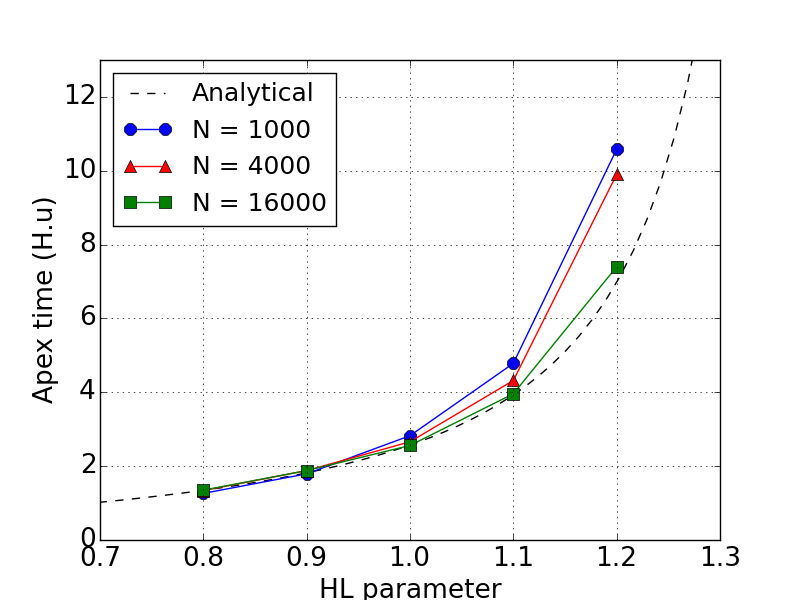
\includegraphics[width=0.6\textwidth]{Figures/2_apextime_NH.png}
\end{center}
\caption[Analytical and simulated apex times as a function of \tHub]{Analytical and simulated apex times as a function of \tHub.}
\label{Fig:2_apextime_NH}
\end{figure} 

We show on Fig~\ref{Fig:2_apextime_NH} the expected analytical curve as a dashed line, then the numerically obtained apex times from our different \tHub and memberships, averaged over all similar runs. The 16k runs follow the analytical expectation within 5\%, while lower membership models take more time than expected to stop expanding at high \tHub, overshooting by as much as 30\% for \tHub =1.2. Visual inspection of the runs showed that low membership models were more susceptible to have a  large clump forming and perturbing the expansion. As we will show in the present section, low-N clusters contains more massive clumps in relative mass than high-N models. When a massive enough clump forms during the expansion, it offsets the matter distribution and skews the half-mass radius (computed from the barycenter of the full system) to higher values, offsetting its fall from the collapse. To reduce unwanted ``sur-fragmentation" effect, we use analytical apex times to select our fragmented configurations.  


\begin{figure}
\begin{center}
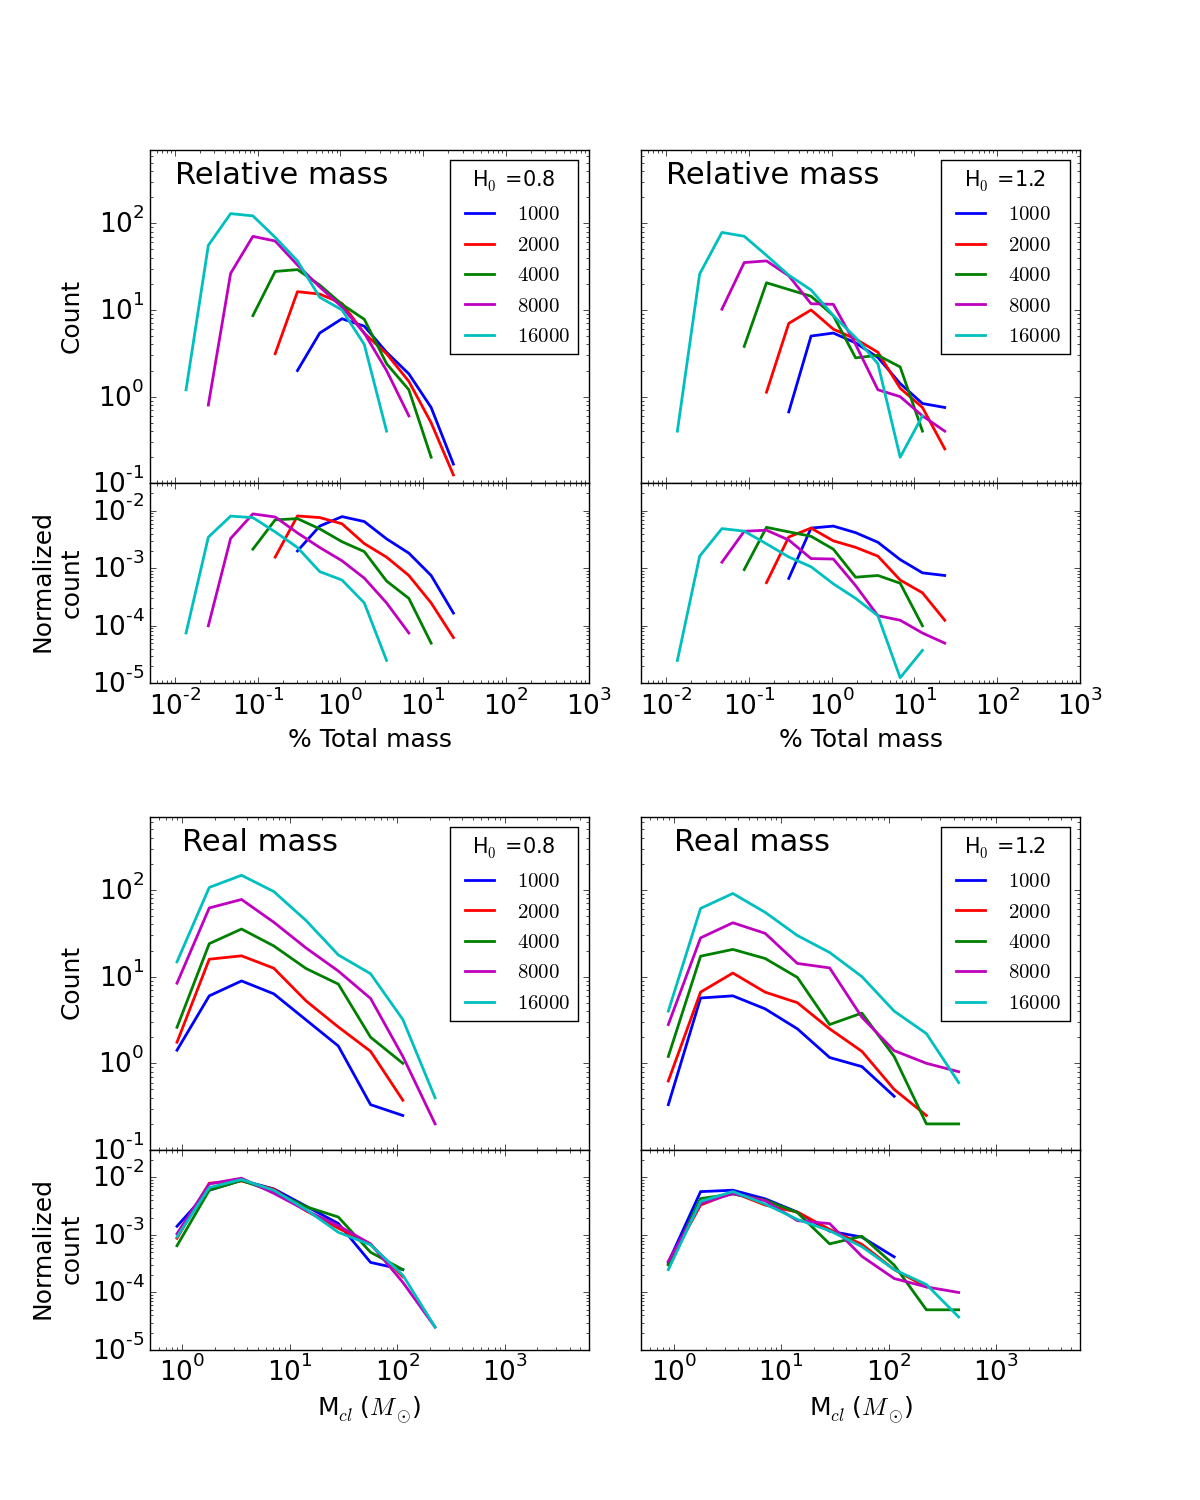
\includegraphics[width=\columnwidth]{Figures/2_ClumpMF_N.png}
\end{center}
\caption[Clump mass function for several memberships and two $\Hub_0$]{Clump mass function for several memberships and two $\Hub_0$. Masses in the top panels are in H\'enon units, the x-axis was scaled with a factor 100 to get a percentage of the total mass of the system. Bottom panel masses are in physical units. In each panel, top sub-panel shows actual clump count in each bin (averaged over sampling), while bottom sub-panel normalize the count by the model membership. }
\label{Fig:2_ClumpMF_N}
\end{figure} 

\begin{figure}
\begin{center}
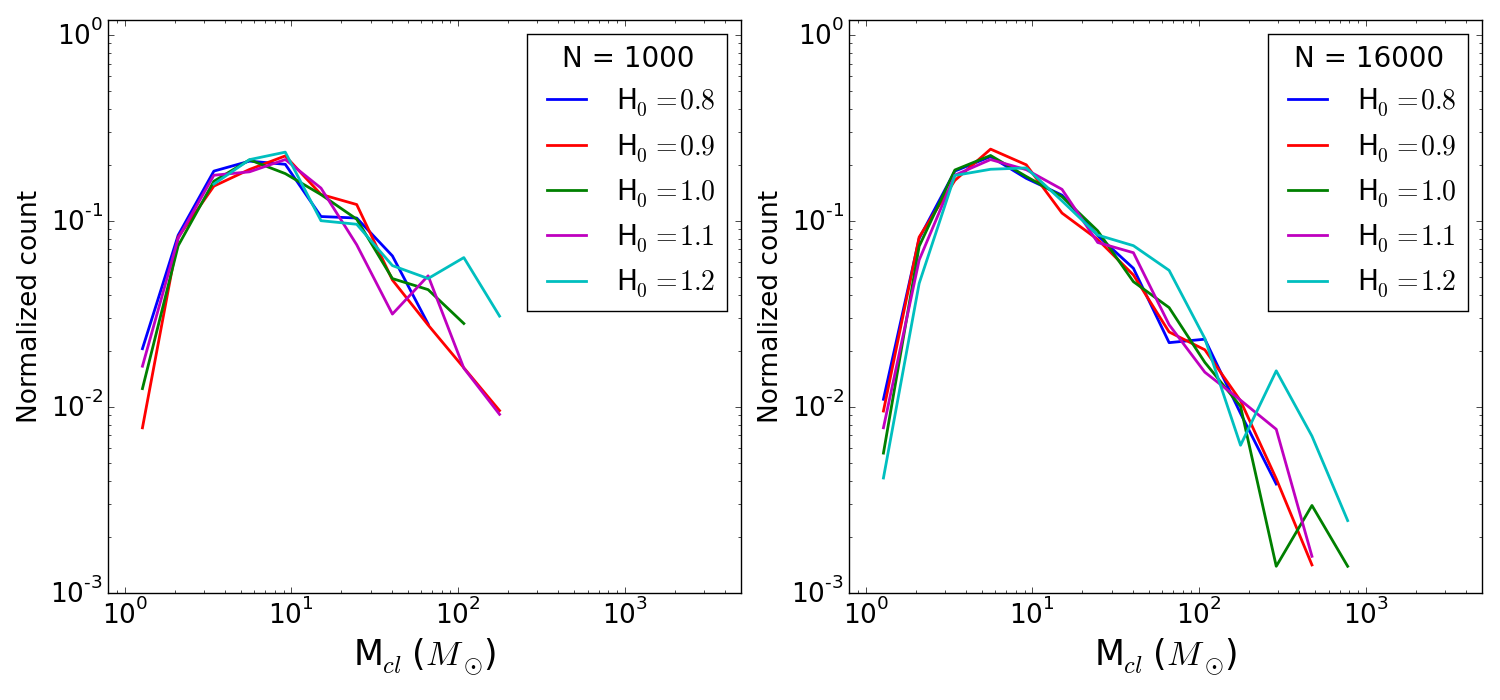
\includegraphics[width=0.95\columnwidth]{Figures/2_ClumpMF_H.png}
\end{center}
\caption[Clump mass function in real mass for several $\Hub_0$  and two memberships]{Clump mass function (real mass) for several $\Hub_0$  and two memberships: N=1000 (left panel) and N=16000 (right panel).}
\label{Fig:2_ClumpMF_H}
\end{figure} 


\subsubsection*{Clump mass function}
 The clump-finding algorithm was ran on the fragmented models to obtain the clump mass function. The results are summarised as histograms on figures \ref{Fig:2_ClumpMF_N} and \ref{Fig:2_ClumpMF_H}. We have used bins of constant logarithmic intervals. We average the results over each model's sampling, hence the histogram can go down to fractional values.
 
 Looking at the top panels of Fig~\ref{Fig:2_ClumpMF_N}, we see the mass function of clumps in \textit{relative} mass, the percentage of total mass they contain.  Clumps in small-N systems tend to contain a much larger portion of the total system mass than in large-N systems, which is even clearer in the normalized count sub-panels. In fact, for \tHub = 0.8, the peak of the mass function for N=1k happens at 1.1\% of total mass, while for N=16k, it happens at 0.07\%. These values ratio gives $\sim$ 16, the membership ratio: the clumps relative masses are inversely proportional to the model's membership.
 
This can be interpreted as a underlying common clump distribution in physical mass, regardless of the total membership of the model. This is confirmed by looking at the bottom panels of Fig~\ref{Fig:2_ClumpMF_N}, in which clump distributions are plotted in physical mass, once the masses of stars have been rescaled from H\'enon units to match the original stellar mass function. Looking at the normalized count subpanels, it is clear that 1k and 16k models have the same clump distribution, when raw count subpanels show clumps are expectedly more numerous in high-N models. The difference between \tHub = 0.8 and 1.2 is not clear from the graph, but it seems a higher \tHub pushes the upper limit of the distribution to slightly higher masses.

To illustrate this last trend, we turn to Fig~\ref{Fig:2_ClumpMF_H} where clump MFs are shown for various \tHub and a common membership. For  both N=1k and N=16k, the distribution preserves its shape for various \tHub, and gets prolonged at higher clump masses for N=16k, as more mass is available to build clumps.

 Thought the distribution does not undergo any dramatic change, a weak trend with \tHub is seen in both panels: as the strength of expansion increases, the distribution slightly decreases at low clump masses and slightly increases at higher clump masses, the pivot mass being $\sim$ 30 $\Mo$. We look at the 16k model and follow the cumulated mass inside all clumps, as well as the percentage of this mass in clumps below and above 30 $\Mo$, for different \tHub:

\begin{center}
\begin{tabular}{l|rrrrr}
\centering
\tHub   & 0.8 & 0.9 & 1.0 & 1.1 & 1.2\\ 
\hline
$M_{tot}$ & 3502 & 3478 & 3582 & 3683 & 3561\\
$ < 30 \Mo$(\%) & 66 & 65 & 55 & 49 & 44\\
$ > 30 \Mo$(\%) & 34 & 35 & 45 & 51 & 56\\
\end{tabular}
\end{center}

From this data, we get two facts about our fragmented models: the mass contained in clumps does not depend on \tHub ($<$2\% dispersion) and there is a transfer of mass from small clumps to more massive ones as the expansion lasts longer.

To summarise: the general shape of the clump mass function is common to all membership and \tHub. In physical mass, the same clumps form in 1k and 16k models, almost regardless of the duration of the expansion. We note a mass transfer from small to high mass clumps when \tHub increases, that is consistent with a merging process: small clumps assemble or get accreted by large clumps. When the initial expansion is strong, the merging lasts longer and more mass is transferred. This is confirmed by visual inspection of the models, as we see clumps merging during the expansion.




\subsection{Influence of stellar mass function}
\label{Sub:2_ClumpMF_MF}




Neither \tHub or N seem to heavily influence the shape of the clump mass function. We now turn to another parameter: the stellar mass function. We know the clumps are seeded by density fluctuations in the initial uniform sphere. These fluctuations are governed by pure Poisson noise in the case of identical stellar masses, but are modified and enhanced once stars follow a mass function themselves: a high-mass star surrounded by lighter ones will by itself introduce a localized strong density fluctuation. We expect a relation between the clump mass function and  the {\it stellar} mass function in the generated initial conditions.

To quantify this relation, we ran a set of simulations where all the stars have the same mass, and two sets for which a Salpeter mass function with $\alpha = 2.35$  was truncated at different upper- and lower-bounds. A total of 15000 stars in a Hubble configuration were used, all let go  with the same initial expansion rate  $\Hub_0 = 1$. For the multi-mass models, the mass range  was chosen as $[0.3, 100]\, \Mo$ and $[0.35, 20]\, \Mo$ so that the mean stellar mass $= 1\Mo$ as for the single-mass models. Thirty different runs were performed in each case and the outcome averaged for better statistics. These are refered to as Rmh1, Rmh100 and Rmh20 in Table \ref{Tab:2_models}.

On Fig.~\ref{Fig:2_ClumpMF_MF}, we display the clump mass function for the truncated Salpeter  models as a red solid line, while the single stellar mass models are shown in green dash. A grey shade indicates one standard deviation where statistics allow ({\it i.e.}, large numbers), and, as in previous section, we have used bins of constant logarithmic mass intervals.  Fig.~\ref{Fig:2_ClumpMF_MF_1} shows Rmh20 models, and \ref{Fig:2_ClumpMF_MF_2} shows Rmh100 models. 
With clump membership restricted to $N \geq 12$, the identical-mass model  stays relatively close to a power law (straight dotted line on the figure) of index $\approx -4$ for the higher mass clumps. A spread in stellar masses leads to much more massive clumps (we counted $\simeq80$ clumps of $12 \Mo$ for the equal-mass case~; and $\approx 32$ with a mass $ \le 12 \Mo$ for the other ones) . This transforms the clump mass function, from a near-power-law, to a bell-shaped distribution.  





 \begin{figure}
\center
    \centering
    \begin{subfigure}[b]{0.49\textwidth}
    	\centering
    	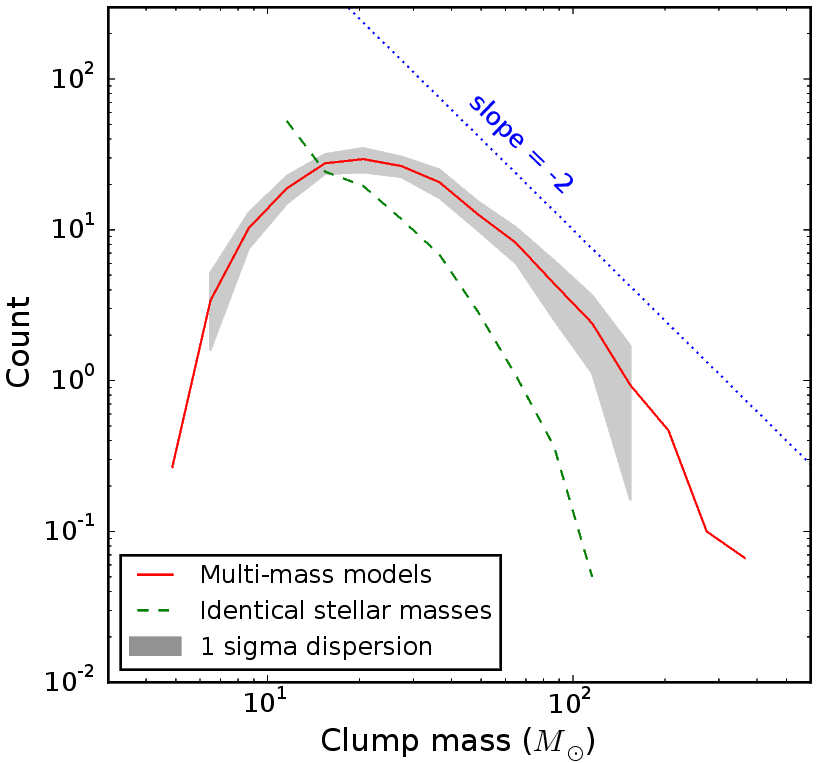
\includegraphics[width=\textwidth]{Figures/2_ClumpMF_MF_1}
        \caption{Stellar mass range $[0.35, 20]\, \Mo$ }
        \label{Fig:2_ClumpMF_MF_1}
    \end{subfigure}
    \begin{subfigure}[b]{0.49\textwidth}
    	\centering
    	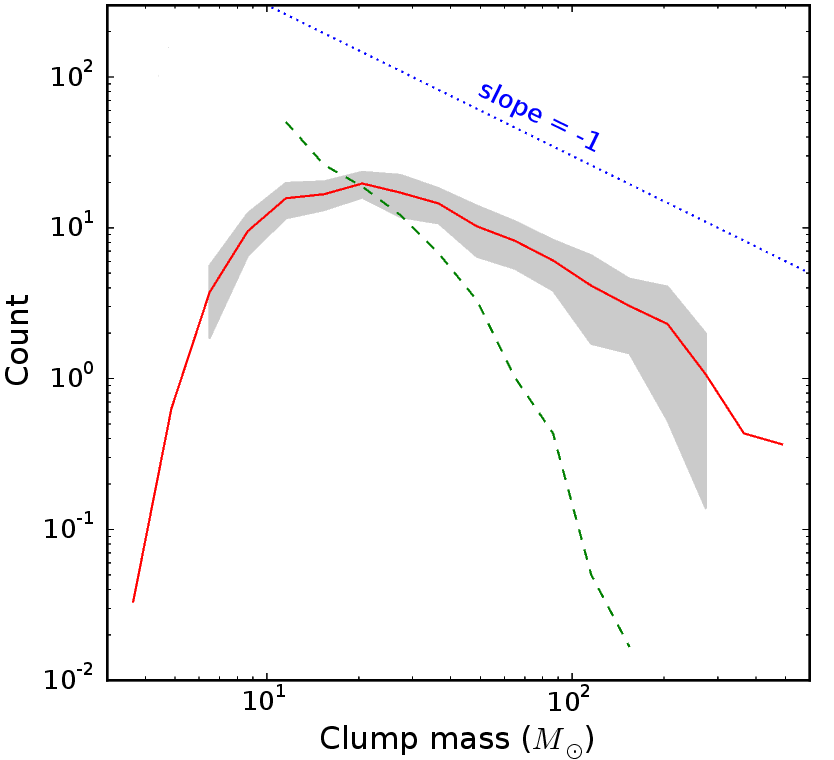
\includegraphics[width=\textwidth]{Figures/2_ClumpMF_MF_2}
        \caption{Stellar mass range $[0.3, 100]\, \Mo$}
        \label{Fig:2_ClumpMF_MF_2}
    \end{subfigure}
\caption[Clump mass functions for $m_{max} = 20~\Mo$ and $100~\Mo$]{Mass function of the clumps identified with the MST algorithm. The calculations all had $N = 15 000$ stars, and we have averaged over 30 realisations for each configuration.  The results for three stellar mass functions  are displayed: a model with equal-mass stars (green dashed line); a Salpeter distribution function truncated at $20 \Mo$ (solid red line, left); a Salpeter distribution function truncated at $100 \Mo$(solid red line, right). (a) The clumps  mass function for equal-mass models  shows a trend with mass roughly in agreement with an $M^{-4}$ power-law. By comparison,  the results for an  Salpeter stellar distribution function  truncated at $20 \Mo$ has a bell-shaped profile, with a peak around $M = 20.5 \Mo$; only the tail-end shows marginal agreement with an $\propto M^{-1.7}$ power-law (dotted line on the figure); (b) another Salpeter distribution function but with  the upper-mass truncation  set at $100 \Mo$. The tail at large clump mass is now much flatter, with a slope $\approx M^{-1}$, (dotted line on the figure as well). The bins used  had constant logarithmic mass intervals.}
\label{Fig:2_ClumpMF_MF}
\end{figure}



When very massive stars are included in the calculations, yet more massive clumps are formed (Fig.~\ref{Fig:2_ClumpMF_MF_2}). The formation of large sub-structures depletes the number of clumps around the peak value, and so the distribution becomes broader and shallower. The mean clump mass for the different cases read $20 \Mo$ (equal-mass), $32 \Mo$ (Salpeter $m_{max} = 20 \Mo$) and $45 \Mo$ (Salpeter $m_{max} = 100 \Mo$), a steady increase with the width of the stellar mass spectrum. On the other hand, the position of the peak of the distribution remains unchanged at (roughly) $20$ to $21\Mo$. The trend in total number of clumps detected is a slight {\it de}crease with the broadening of the  stellar mass spectrum, from 187, down to 151 respectively for the $m_{max}=20$ and $100 \Mo$ Salpeter models.  
%  Much of this difference in the  number of clumps is accounted in the 
 % range 0 to $20 \Mo$, for which 73 and 54 clumps were found, respectively. 
% The fractional decrease of 26\% compares well with the lower number of stars in the interval 
% $[10,20]\Mo$   for the model with the broader mass spectrum (which reaches $20\%$).  
  We observe that the overall fraction of  stars found in clumps (some $\approx 6500$ out of 15000, or 43\%) stays unchanged.
  
We argue that the shape of the clump mass spectrum provides indirect evidence for the predominant role of massive stars as seeds for overdensity growth in our simulations. This is to be opposed to a full hierarchical build-up of clumps from very tiny sub-structures. There are two tell-tale signs to support this view~: a) if high-mass clumps formed through the repeated and stochastic merger of small clumps, then the clump mass function should tend to a log-normal distribution, which is  symmetric (in logarithmic scales) with respect to the peak value, whereas the distributions shown here lack this basic property~; and b) the ratio of maximum clump mass to mean mass may exceed 15 when the  stellar truncation mass is set to $20\, \Mo$, and reaches only $\sim 4$ in the case when the upper mass is set to $100\, \Mo$. If small-ish clumps were merging at the same rate in both models, then this ratio should be comparable. Instead, very large clumps take too long to assemble and the merger rate drops with clump mass. Recall that all fragmentation calculations ran for the same total time. There is a weak merging process happening, as shown in the previous section, but it is marginal, as heavy clumps likely form from massive star seeds.

To check this hypothesis, we borrow from black hole dynamics in galactic nuclei the notion of a {\it radius of influence}, which is the radius  enclosing as much mass in the stars as the central black hole mass (see e.g. \citealt{Merritt2013}).  Here, the stars inside the influence radius are bound to the massive star at the centre. Thus if a massive star is a seed for a clump, and only the stars inside the influence radius remain bound to it, we should count as many clumps in the mass range $2m_\star, 2 m_\star + 2{\rm d}m_\star$, as there are stars in the range $m_\star, m_\star + {\rm d}m_\star$.  The maximum clump mass exceeds twice that of the most massive stars $m_{max}$, which implies some degree of merging and is consistent with the previous section. If we count all clumps starting from the truncation value $m_{max}$ of the stellar mass function,  
%presume that the clumps all formed from fragments seeded with a massive star and its cortege of bound stars, 
then we should find as many clumps in the mass range above $m_{max}$, as there are stars in the interval $[m_{max}/2, m_{max}]$.  We find for runs with $m_{max} = 20 \Mo$ some $120$ clumps more massive than that, when there are $\simeq 100$ stars in the range $[10, 20] \Mo$; and some $14$ clumps of $100 \Mo$ or more, when there are (on average) 9 stars in the mass range $[50, 100] \Mo$. This calculation suggests that  most massive stars act as seeds for the formation of large clumps in the generated initial conditions.













\section{Clump contents}

In this section we compare the clumps derived from the \HubLem expansion method with the distribution of proto-stars that form in hydrodynamical simulations and with observations of young star forming regions. We first look at the velocity field inside and outside the clumps, then we investigate the stellar content of the clumps themselves and their mass segregation.


\subsection{The velocity field}
\label{sec:velocityfield} 




 \begin{figure}
\center
    \centering
    \begin{subfigure}[b]{0.49\textwidth}
    	\centering
    	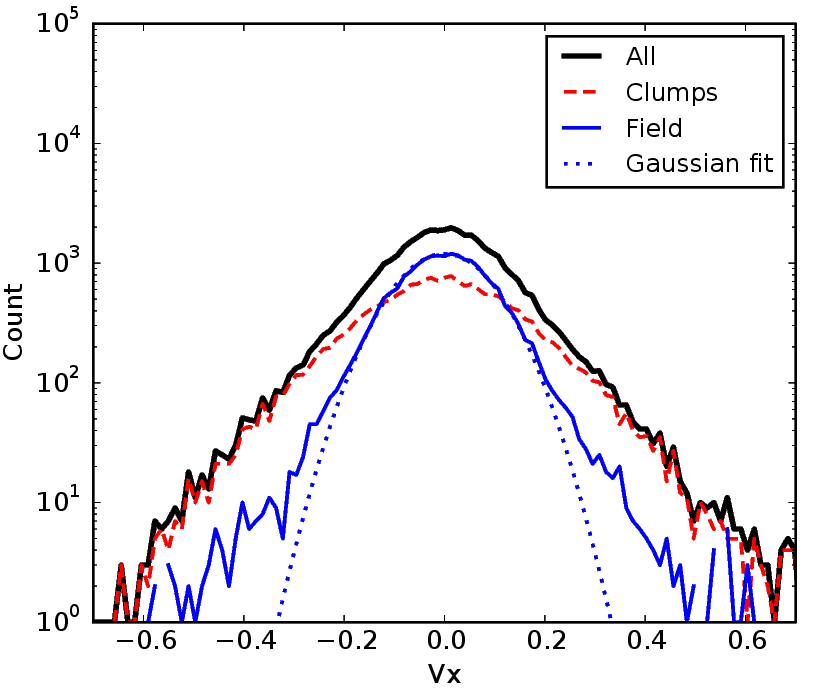
\includegraphics[width=\textwidth]{Figures/2_Vx_histogram_1}
        \caption{Distribution clumps/field}
        \label{Fig:2_Vx_histogram_1}
    \end{subfigure}
    \begin{subfigure}[b]{0.49\textwidth}
    	\centering
    	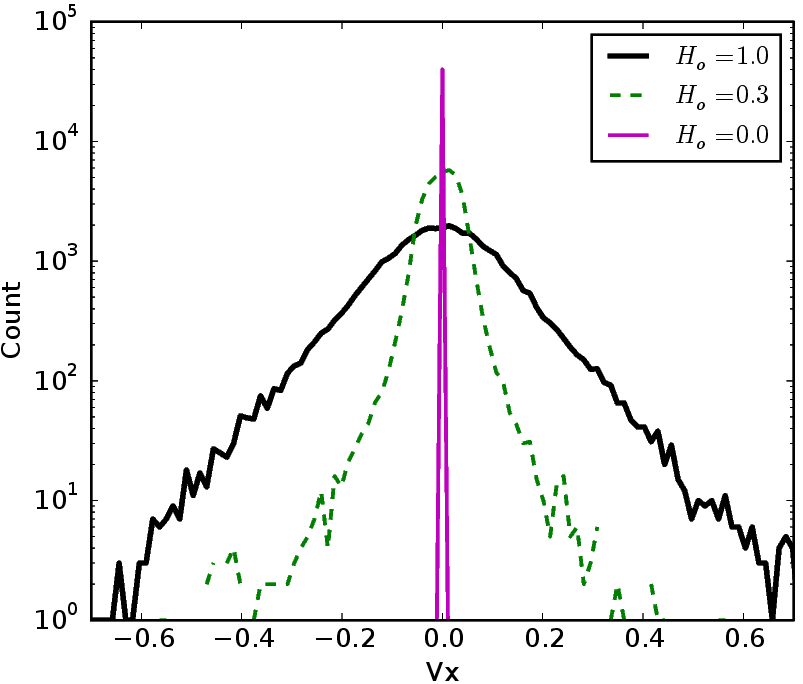
\includegraphics[width=\textwidth]{Figures/2_Vx_histogram_2}
        \caption{Distribution for different \tHub}
        \label{Fig:2_Vx_histogram_2}
    \end{subfigure}
\caption[One-dimensional velocity distribution of clump members and field stars]{(a) Distribution of the one-dimensional velocity field for the whole cluster as the thick solid black line, in the simulation labelled as R40h20 at the apex time (H$ = 0$). The red dashed distribution shows clump members and thin solid blue the field particles. (b) The distribution for three different values of \tHub: when $\Hub_0 = 0$, the distribution is a Dirac-$\delta$ around $v = 0$. The central distribution broadens as \tHub increases to 0.3 and 1. Velocities are in H.u..} 
\label{Fig:2_Vx_histogram}
\end{figure}




 There is no hydrodynamics in the approach that we have taken, nevertheless expansion under gravity alone is equivalent to the adiabatic expansion of gas~: for that case, the first law of thermodynamics equates the drop in internal energy ${\rm d}U$ to minus the external work,  $-p {\rm d}V$. At constant mass, the change in gravitational energy ${\rm d}W$ is $ - {\rm d}E_k$, where $E_k$ is the kinetic energy. With $W < 0 $ but increasing over time, this implies that $E_k$ drops in amplitude. In the case when the motion is strictly radial, $E_k = 0$ when $H = 0$ and all stars come to rest. We ask to what extent the growth of substructures and non-radial motion  off-set the `adiabatic cooling' brought on by expansion. 

Fig.~\ref{Fig:2_Vx_histogram_1} graphs the x-axis one-dimensional velocity distribution for the R40h20 model. The left-hand panel displays the overall distribution as well as the two sub-populations of clumps members and out-of-clump \textit{field} stars. We identified some 20944 stars in clumps (or $\approx $ 52\%) at the end of expansion. The overall spherical symmetry is validated by the peak in the distribution around $v_x = 0$.

As sub-structures form and  interact mutually, generating tangential as well as radial motion, the peak broadens but remains symmetric about the origin.  The large velocities are brought by stars in clumps, which demonstrates that interactions within the substructures boost the internal velocity dispersion of the cluster as a whole. Field stars dominate the low-amplitude regime. Their velocity distribution is well-fitted with a  Gaussian (shown as a dotted blue line), down to one-tenth the height of the central peak, or about 1\% of all field stars. 

To illustrate further the idea that large velocities are confined to clumps formed by fragmentation modes, we compare on Fig.~\ref{Fig:2_Vx_histogram_2} a set of fragmented models 
with different initial  values of  $\Hub_0$: 0, 0.3, and 1. 
Clearly when $\Hub_0=0$, the velocities are identically zero and there is no fragmentation whatsoever (apart from root-N noise). The distribution is then a sharp peak centered on zero. For positive but low values of $\Hub_0$, the fragmentation modes do not develop much before the apex and the (non-radial) velocities remain small. The central peak  has a much narrower dispersion, and the high-velocity wings are clipped. In this case, too, analysis of the  weakly fragmented system shows that virtually all high-velocity stars are found in clumps. The velocity distribution for the case  $\Hub_0 = 1$ is added for comparison. The fact that the full range in velocities is reduced by a factor $\sim 3$ for the 
less fragmented model is also an indication of the shallower potential well of the clumps

The full population velocity distribution (solid black line) at first sight is very similar to those of \citet[Fig.~5]{Klessen2000}. In that figure, the authors show the velocity distribution of gas particles in a fragmenting system. \citeauthor{Klessen2000} attribute the high-velocity tails to gas particles falling towards stellar clumps at supersonic speed. Supersonic motions imply that gas particles trace ballistic trajectories, and hence behave like point mass particles. 

A small fraction of field stars in our calculations also have large velocities. We suspected that these stars might have acquired their large velocities through in-fall toward a nearby stellar clump. We did not, however,  find compelling evidence that would allow us to identify the origin of high velocities in field stars. Inspection of a sequence of snapshots failed to show that the velocity vectors were pointing at nearby stellar clumps: it is therefore not possible to make the same assertion as \citeauthor{Klessen2000} and state that stellar clumps accrete some field stars.

It is possible, on the other hand,  that high velocities originate from past star-star interactions. However, we did not find clear trends in the few orbits that we studied which would confirm such an event. The question of mass accretion by stellar clumps might be best settled if we added gas to our simulations to boost the mass resolution, and analysed model data using mock CCD frames, as did \citeauthor{Klessen2000}. This was not attempted here.

We close this section with a remark about the velocity distributions seen on Fig.~\ref{Fig:2_Vx_histogram} and the internal state of the stellar clumps. Because small clumps would have time to evolve dynamically through star-star collisions and reach a state of near-equilibrium (see \S\ref{Sec:Timescales}) we would expect clumps to develop a velocity field similar to Mitchie-King models of  relaxed self-gravitating star clusters \citep{BT}.  The one-dimensional velocity distribution of Mitchie-King models plotted in a logarithmic scale approaches a flat-top when $|v_{1d}|$ is small,  and cuts off rapidly at large values~: the distributions are  concave at all velocities. This holds true for all models independently of their King parameter\footnote{Notice how this holds only because of the choice of a logarithmic vertical axis.} $W_0$. 

The shape of the distributions displayed on Fig.~\ref{Fig:2_Vx_histogram}, on the other hand, is convex as we shift, from small, to large $|v_{1d}|$. We deduce from this straightforward observation that the clumps that formed through fragmentation and subsequent mergers cannot be treated as fully in isolation and in dynamical equilibrium \`a la Mitchie-King.  Fragmentation in hydrodynamical calculations often proceeds from filaments and knots  (e.g., \citealt{Klessen2001,MacLow2004,Maschberger2010,Bate2014}). The clumps that form in a fragmenting  Hubble  flow are also surrounded by filaments and other structures which perturb them.




\subsection{The stellar mass function in clumps} 



We show on Fig.~\ref{Fig:2_ClumpMembers} the mass function of stars in clumps, field and in the whole cluster. For brevity, we only show a model with a mass function truncated at $20 \Mo$, Rh20,  however our conclusions are not sensitive to the truncation value. The mass function of $\approx 6400$ stars that were found in clumps (some 43\%) is displayed as the red solid curve and all other stars, field stars, as the blue solid curve. The theoretical Salpeter distribution function for the same number of stars is shown in black dots, with grey shades giving the  $1 \sigma$ dispersion from multiple samplings. Finally, the green dashed curve  shows the mass distribution of all 15 000 stars in the model. The lower panel is the same data normalised to the Salpeter data. 

The uptake  in massive stars for the whole population (green dashed line) of both clumps members and field stars is a statistical artefact and lies within the standard deviation of a Salpeter distribution with comparable sampling number. 

The clump member population clearly deviates from a Salpeter distribution in two ways~: first we note a deficit of low mass stars with respect to the theoretical Salpeter; secondly, although a Salpeter mass function is more or less consistent with the population up to $M\approx 2\Mo$(black dotted line) the distribution shows a clear excess of massive stars. We find that practically all the stars more massive than 10$\Mo$ ended up in a clump (this is the point where the solid red curve joins the dash green one). 

A log-log linear regression fit of the clump members mass function gives a power-law index of $-2.15 \pm 0.02$, shallower than the Salpeter index of -2.35. Applying the same analysis to field stars,  we find a steeper mass function of index $-2.46 \pm 0.02$. The difference of $\approx 0.3 $ between the two populations is very similar to what is found in the Milky Way disc (see e.g. \citealt{Czekaj2014,Rybizki2015,Bastian2010} )

\begin{figure}
\begin{center}
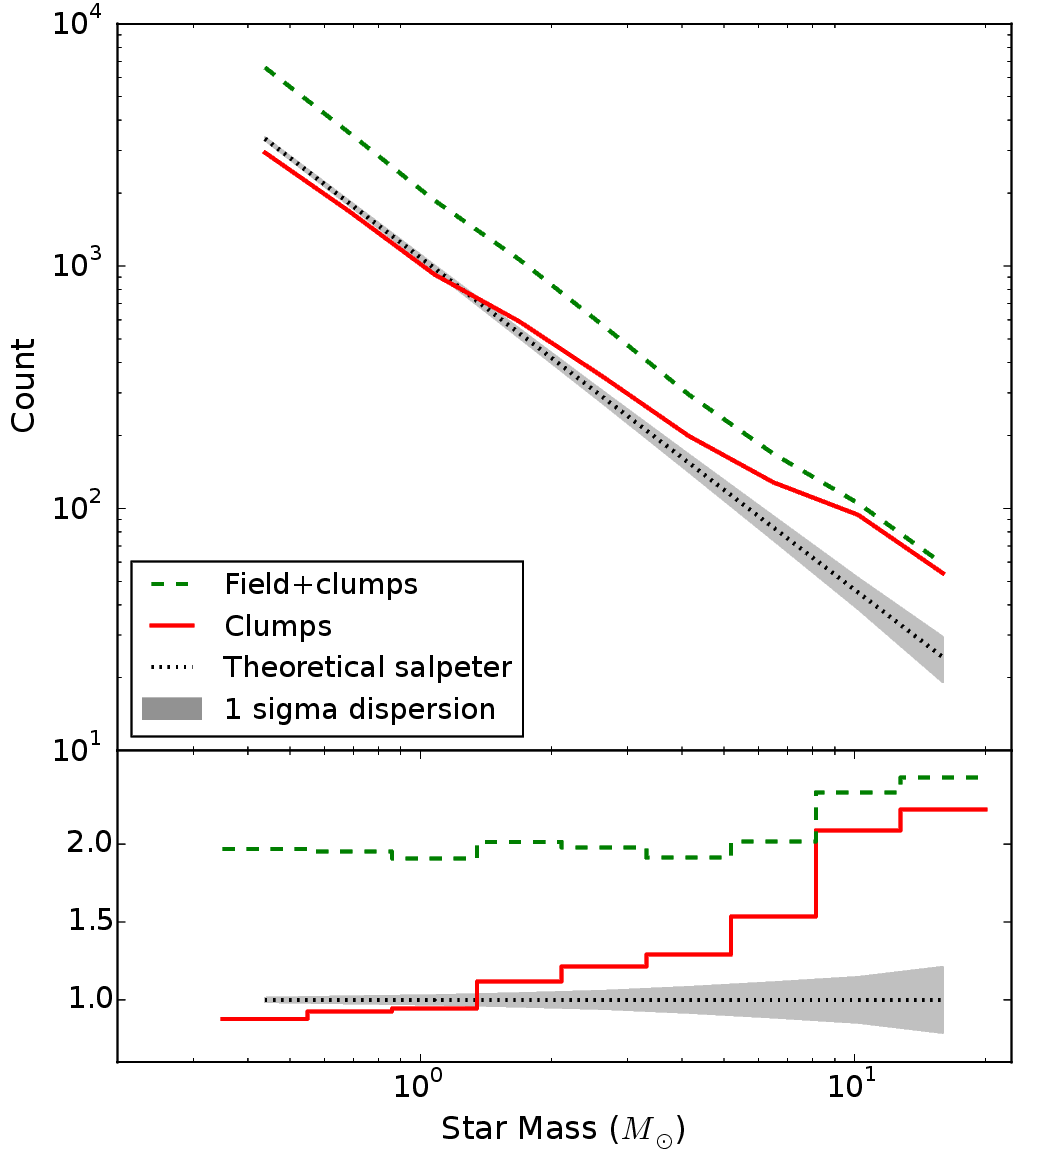
\includegraphics[width=0.69\textwidth]{Figures/2_ClumpMembers}
\caption[Clump member and field stars mass functions]{Top panel~: Mass function of all stars belonging to a detected clump (solid red) and field stars (solid blue). The expectation drawn from a Salpeter distribution function for the same total number of stars in dotted black~; the grey shade are $1\sigma$ uncertainties. The green dashed line is the  distribution for the full cluster. Bottom panel~:  same data normalised to the Salpeter expectation.}
\label{Fig:2_ClumpMembers}
\end{center}
\end{figure}

\cite{Bonnell2004} and \cite{Maschberger2010} showed from inspection of  hydrodynamical simulations that massive stars play a key role in the assembling process of clumps, attracting already formed protostars to them. We find  a similar general trend in Hubble-fragmented gas-free simulations: clumps develop around massive stars so that their stellar mass function is top-heavy. 

This excess can also be seen in the top panel of Fig.~\ref{Fig:2_MaxMass} in which for each of 440 clumps of the R40h100 model, we show as white dots the mass of their heaviest star as a function of the host clump's mass. For comparison, we sampled a Salpeter mass function, drawing the same number of stars as found in each clump. We then identify the most massive star in the Salpeter sample~; the procedure was repeated 15000 times {\it for each clump} to obtain suitable statistics. The color map shows the resulting distribution.



 \begin{figure}
\center
    \centering
    \begin{subfigure}[b]{\textwidth}
    	\centering
    	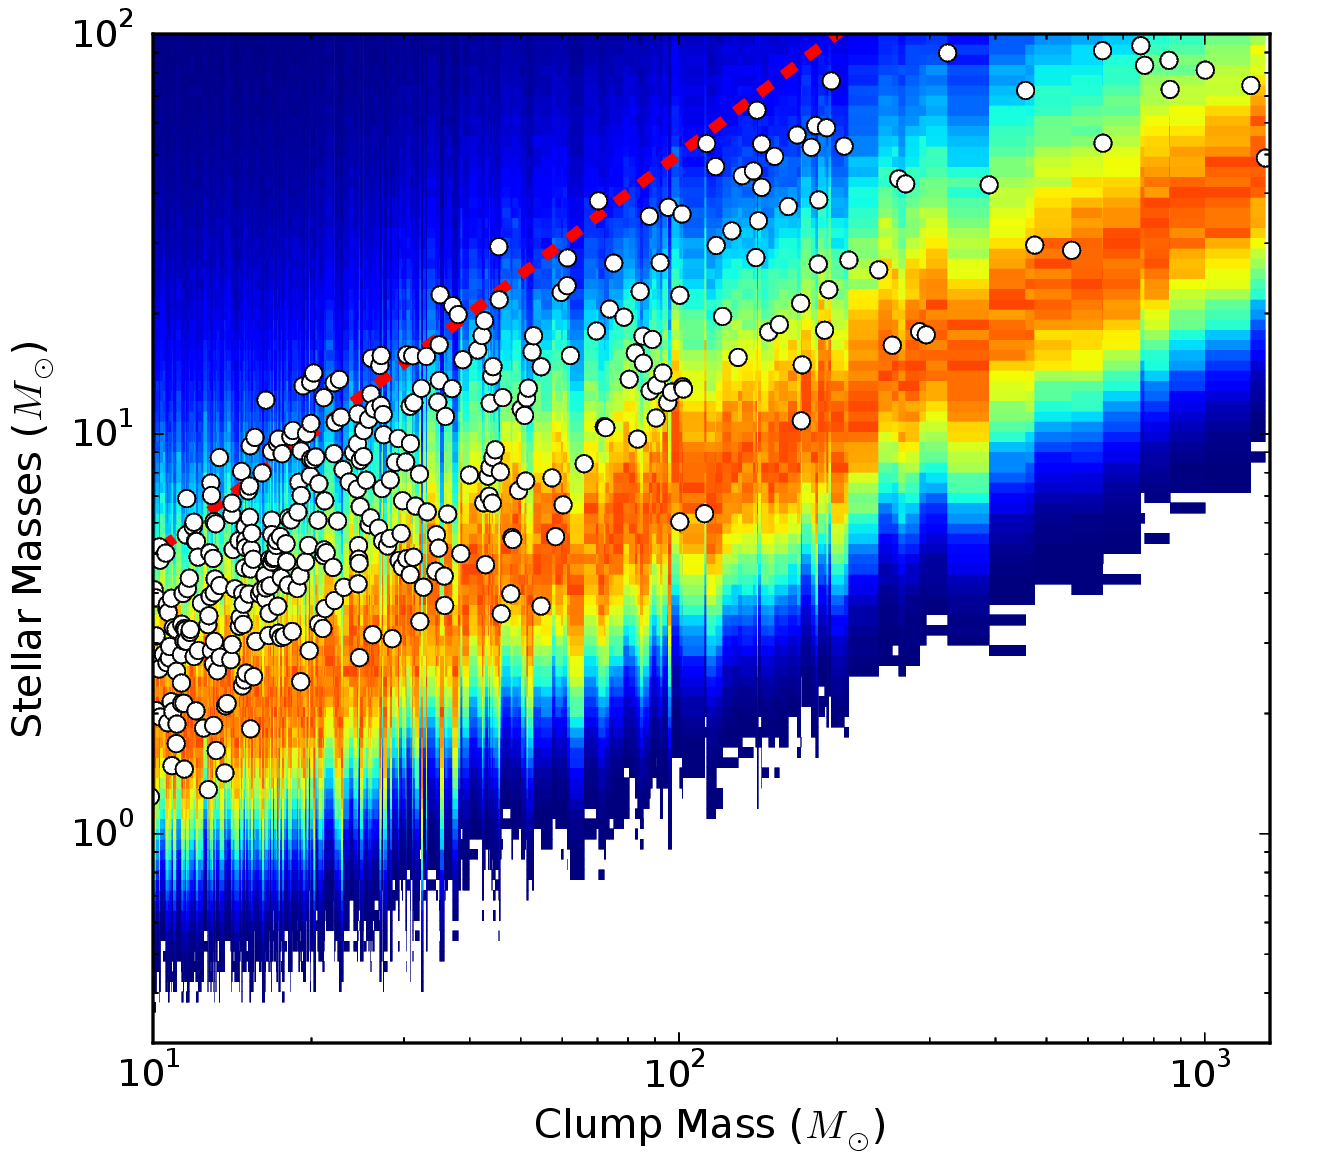
\includegraphics[width=0.7\textwidth]{Figures/2_MaxMass}
        \caption{Distribution clumps/field}
        \label{Fig:2_MaxMass}
    \end{subfigure}
    \begin{subfigure}[b]{\textwidth}
    	\centering
    	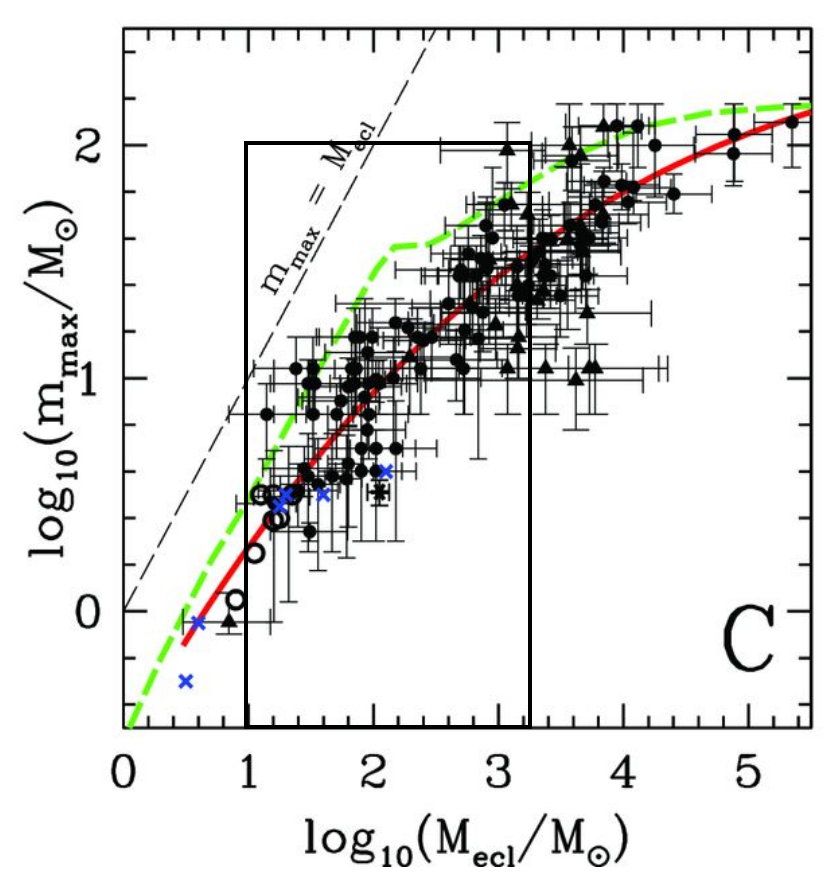
\includegraphics[width=0.6\textwidth]{Figures/2_weidner}
        \caption{Distribution for different \tHub}
        \label{Fig:2_weidner}
    \end{subfigure}
\caption[$M_{clump} - m_{max}$ relation for HL clumps and observed embedded clusters]{(a) Mass of the heavier star in each clump, shown as white dots, as a function of clump mass. The color map shows the likelihood for the maximum mass if all clump members were  sampled from a Salpeter IMF~; the orange crest gives the maximum likelihood. The red dashed line shows the  relation $m_{clump} = 2 m_{max}$ (see. section \ref{Sub:2_ClumpMF_MF}). The data was taken from the R40h100 run. (b) is a similar distribution from \protect\cite{Weidner2013}, built with data about young embedded star clusters from \cite{Weidner2010}. The black frame notes the range of masses displayed in (a). } 
\label{Fig:2_McMmax}
\end{figure}


 In a nutshell, Fig.~\ref{Fig:2_MaxMass} shows for each clump the likelihood that their most massive stars may be drawn from a Salpeter function. One could call the red maximum likelihood zone the "Salpeter valley". Only clumps with a mass $> 10 \Mo$ are included to account for a possible bias when clump membership reaches below $N_d =12 $ stars. It can be seen on the figure that the scatter of white dots tends to lie systematically above the Salpeter valley. If we add the  relation $m_{clump} = 2\max\{m_\star\}$ (cf. section \ref{Sub:2_ClumpMF_MF}), we find some overlap with the data (see the red dashed line on Fig.~\ref{Fig:2_MaxMass}). This clearly illustrates the tendency for massive stars to act as seeds when the clump form, while the scatter is driven by the merger and accretion history of individual clumps. 
 
 The correlation displayed on Fig.~\ref{Fig:2_MaxMass} is in good agreement with observational data for young embedded clusters of the same mass range published by \citealt{Weidner2013}. We reproduced their figure on Fig.~\ref{Fig:2_weidner} with a black frame representing the range shown on Fig.~\ref{Fig:2_MaxMass}. 
 
 Note how the {\it scatter} in the correlation brought on by the dynamical processes at play during the adiabatic fragmentation phase also compares well with the data. Thus the stellar clumps modelled here recover an important characteristic of observed embedded young clusters.
 





\subsection{Mass segregation}
\label{Sec:2_ClumpSegregation}

In this section, we ask whether the clump assembling process at play in our simulations accounts for the mass segregation measured  in  star-forming cores in hydrodynamical simulations. The measure of mass segregation of \cite{Olczak2011} based on the MST, while efficient, will give noisy results for very small-N clumps. Instead, we follow \cite{Maschberger2010} and rank clump members according to their distance to the geometric centre of a clump, which is calculated by number-averaging (so this centre is not the clump barycentre). We then sort the bodies by mass and tabulate the radial rank of the three most massive ones. This process is illustrated on Fig.~\ref{Fig:2_radial_ranking}.


\begin{figure}
\begin{center}
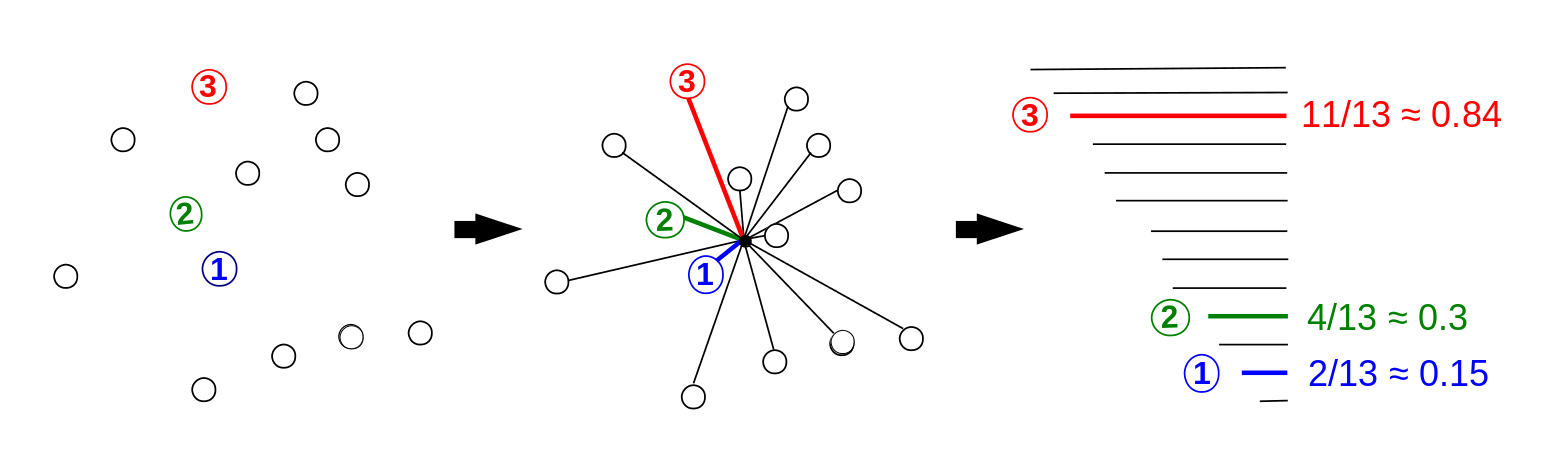
\includegraphics[width=\textwidth]{Figures/2_radial_ranking_schema}
\caption[Illustration of the radial ranking method]{Illustration of the radial ranking method. Stars marked 1,2 and 3 are the first, second and third most massive stars in the clump. Distances to the geometrical center are computed then sorted. The position in the sorted list is converted to a number, the radial rank.}
\label{Fig:2_radial_ranking}
\end{center}
\end{figure}

The great advantage of this approach is that it is independent of geometry and absolute size once the ranking is normalised to the clump membership $N_c$.  One issue arises with the binning of the rank, since small values of $N_c$ give large intervals by construction, and conversely for populous clumps~: we found a good compromise by setting the width of each bin to 1/20 since the mean clump mass $\sim 20 \Mo$ implies $N_c \sim 20$ on average. The procedure is repeated over all clumps identified in the run (typically on the order of $\sim 200$). The diagnostic for an un-biased sampling is a profile with radius that remains the same regardless of the mass selected~; if, furthermore, the stars are (on the mean) un-segregated in radius, then the profiles will be flat. 


Fig.~\ref{Fig:2_ClumpSeg} graphs the  distribution of rank of the three most massive stars in all the clumps from the R40h100 fragmented state. The salient features are that 1) none of the distributions are flat, all three peaking significantly  at small ranks~; and 2) there is a clear trend for the most massive star also to be the most  segregated. Precisely this result had to be expected from the internal dynamics of small clumps (cf. section~\ref{Sec:Timescales}).  Our Fig.~\ref{Fig:2_ClumpSeg} should be compared with Fig.~13 of \cite{Maschberger2010}: the authors also found radial rank distribution to peak at small values for massive stars, showing a level of mass-segregation in their clumps.

It is striking that the measure of mass segregation attained here for a gas-free configuration is a good match to a full hydrodynamical setup. The initial configuration that we have adopted relies only on density fluctuations to seed clumps, however once again we find evidence that massive stars begin and remain the centre of gravitational focus for clump formation. That is not so when clumps are setup using a fractal approach \citep{Goodwin2004,Allison2009}. There is then no segregation initially, and it all develops at or shortly prior to the global system evolution towards equilibrium (the collapsing violent relaxation phase). 


\begin{figure}
\begin{center}
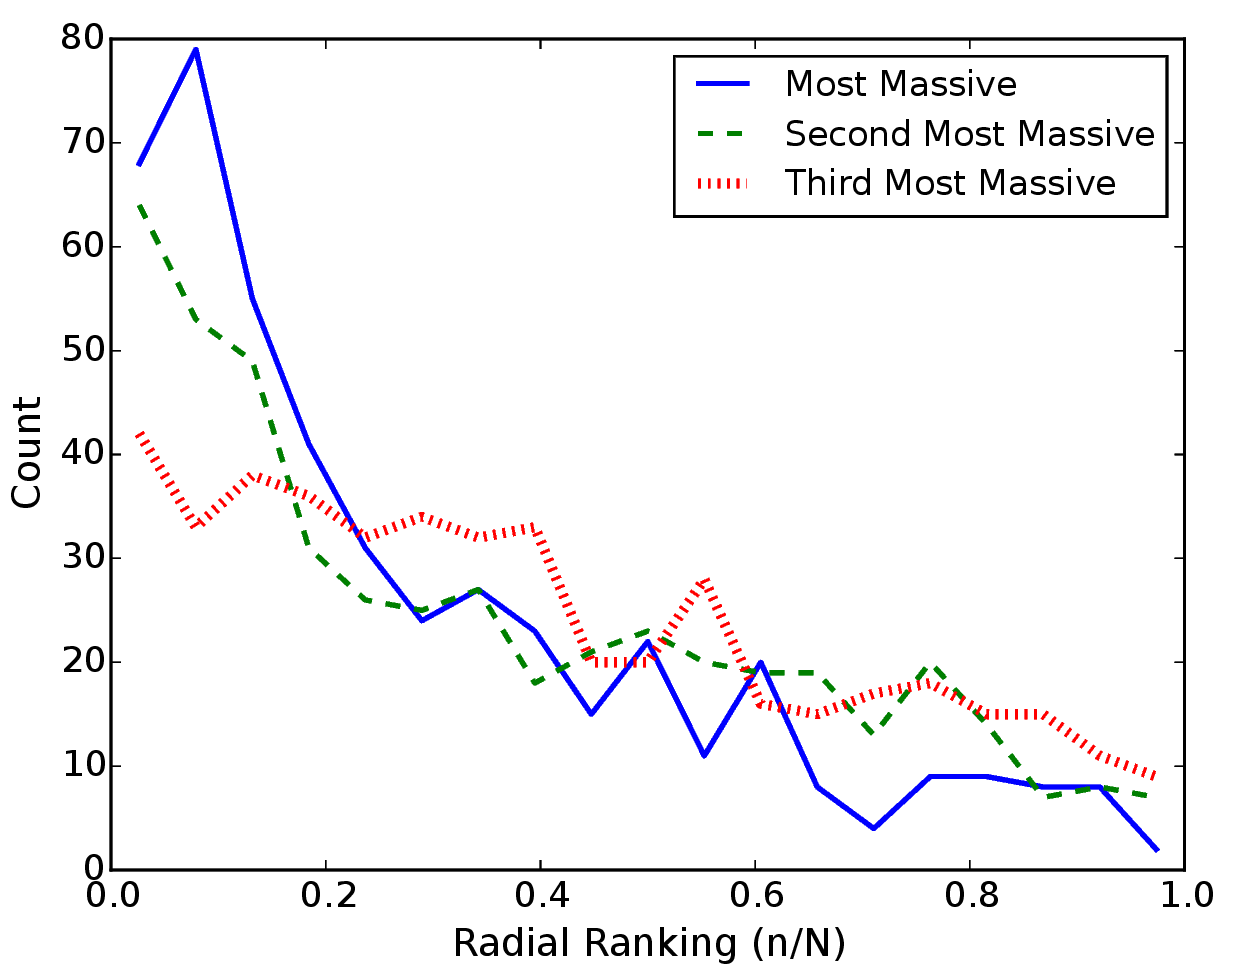
\includegraphics[width=0.6\textwidth]{Figures/2_ClumpSeg}
\caption[Radial ranking of first, second and third most massive stars in each clump]{Histograms of radial ranking of first, second and third most massive star in each clump for a model with N = 40 000 stars (R40h100).}
\label{Fig:2_ClumpSeg}
\end{center}
\end{figure}







\section{Concluding remarks}
\label{Sec:2_conclusion}

We have developed a new approach based on adiabatic fragmentation to set up self-consistent configurations for stellar dynamics that link up the velocity field of stars to their irregular space configuration of arbitrary geometry, such as knots or filaments. The method offers great advantages: it is easy to implement; it can treat an arbitrary number of stars without any resolution issue. The light computational load allows for statistical ensemble averaging over large samples, as was done throughout this chapter. For instance, the computation time on a single card for 80,000 stars is about 12 hours. The methods has its limitations: the most significant one is the failure to include hydrodynamical effects. In the introduction, we mentioned other approaches partly based on hydrodynamics: such hybrid methods have been successful but remain limited in scope, for instance \cite{Moeckel2012}, or demanding in computational resources (and so constrain the number of realizations), as in \cite{Fujii2016}. 

\subsection*{The importance of massive stars}


During the fragmentation process in our models, heavy stars act as seeds for the growth of stellar clumps, and so the stellar clumps mass spectrum is shaped by the mass function of the available {\it stars}. Although the fragmentation through gravitation only does not include the detailed physics of star formation, we noted that hydrodynamical calculations including gas pressure and turbulence suggest that the gravitational potential of massive stars attract more gas and stars and, as such, act act as seeds for the formation of clumps \citep{Bonnell2004}. We therefore recover a key prediction of hydrodynamical simulations. It is then interesting to ask whether observations show a correlation between the host clump mass and its population of massive stars.

 Based on analysis of our fragmented Hubble models, we recover on Fig~\ref{Fig:2_McMmax} a correlation between the maximum mass of a star found in a clump of a given mass, $M_c$. This $\max(m_\star) - M_c $ relation is eerily similar to the compilation for young clusters by \citet{Weidner2013}, from which we extracted the figure \ref{Fig:2_weidner}. Furthermore, we also found that the stellar mass function in clumps has a much flatter (top-heavy) profile than in the field, {\it i.e.} stars that do not belong to any clump: power-law fits for the two stellar populations show that the Salpeter index for clumps stars is lower by about $\approx 0.3$ compared to the same index for field stars. A similar difference is deduced for Milky Way data ( \citealt{Czekaj2014,Rybizki2015}; see also Fig 2 from \citealt{Bastian2010}):  we argue that these characteristics will help tighten our understanding of the long-term evolution of such stellar associations, given that their properties are, on the out-set, close to actual data for young clusters. It should be emphasised that the global index of external galaxies may differ significantly from the canonical value $\alpha = 2.35$ ({\it e.g.}, the GAMA survey, \citealt{Gunawardhana2011}; see also \citealt{Hoversten2008}). We have not explored here to what extent this difference in indices  between field and clump populations will change for other values of the global index $\alpha$.

We have also noted that the clumps are {\it mass segregated} at birth, i.e. at the end of the fragmentation process. When we apply the same ranking statistics as for hydrodynamical calculations of star formation, we obtain the same level of segregation for the three most massive stars in a clump (cf. Fig. \ref{Fig:2_ClumpSeg}). %Heavy or light stars caught in dense clumps have high velocities, while  only a small fraction of field stars have such large velocities: we found that the velocity distribution function of field stars is well fitted with a Gaussian, except for the $\sim 1\%$ with the most extreme velocities. We drew a comparison with the SPH calculations by \cite{Klessen2000}, who attributed the high-velocity tail of gas particles to their in-falling onto stellar clumps. However, we could not identify unequivocally the origin of the large velocities for the field stars (past star-star interactions, attraction by a clump, .. ). That point may well be worth exploring in a future study, as it relates to the likelihood of accretion of field stars by a dense stellar clumps. Recent SPH calculations by M. Bate and collaborators hint at continued exchanges between stellar cores and their environment.

\subsection*{The slope of the clump mass function}

\cite{Klessen2000,Klessen2001} fit the gas clump mass function of their simulations with a power-law $\frac{dN}{dM} \propto M^{-\beta}$ where $\beta \simeq$ -1.5. On the other hand, the \textit{cluster} mass function in the Milky Way can be described as a power law with an index ranging from -2 to -2.4 \citep{Haas2010}. We have indicated that a power-law relation with a slope $ \beta \simeq -4$ is a rough fit for the case where all the stars are identical (Fig.~\ref{Fig:2_ClumpMF_MF}). This is not so  when a stellar mass spectrum is included~: if a Salpeter distribution function is truncated at $20 \Mo$ a power-law with slope $ \beta \simeq -1.7$ still fits approximately the distribution of clumps of  mass $ > 20\, \Mo$~; and when the Salpeter distribution function is truncated at $100 \Mo$, a power-law similarly fits the tail-end of the distribution but now with a slope of $\simeq -1$ (see Fig.~\ref{Fig:2_ClumpMF_MF_2}). It is intriguing that the slope of the distribution should fall within the bracket of values for the observational data for clusters ($-2.4^+$) and hydrodynamical fragmentation models (-3/2). If the clumps formed from hydrodynamical fragmentation should become individual star clusters, and recover the $\beta \simeq -2 $ or lower slope of observational data, then the distribution function must become steeper and also cover a broader range of masses. The same conclusion applies to the Hubble clump distribution function.

This implies either that clumps will merge so that a few very massive clusters will emerge, or that fewer massive clumps form in the first place. Comparison with existing cluster population needs us to assume these clumps do not fall back and merge through collapse. This is possible with an adequate galactic tidal field ripping apart this fragmented configuration and isolating the clumps before the collapse. Many of the small stellar overdensities detected as clumps would not survive more than a few million years before dispersing through collisional evolution, however the larger clumps could survive and appear as isolated clusters or part of an association. These massive clumps   are the key to comparison to the galactic cluster mass function. We have shown how the stellar IMF provides seeds for the growth of massive clumps and have illustrated this with a Salpeter power-law IMF. A more realistic  IMF has a steeper power index at larger stellar masses \citep{Kroupa2002,Chabrier2005}. The fragmentation of stellar systems with fewer massive stars would deplete the clump mass function at larger masses more in line with observed statistics for clusters. 
This variability in the clump mass function highlights the major influence of the stellar IMF on the fragmentation process. A full exploration of fragmentation requires hydrodynamical simulations, which we have not performed here. These simulations remain limited to much smaller systems \citep{Bate2014,Lomax2014}.

\paragraph*{}
In the next chapter we assume an absence of tidal field and follow through with the final stage of evolution towards equilibrium. We compare the final configuration with those of \cite{Allison2009} and the recent study by \cite{Caputo2014}. 
